\documentclass[parskip, twoside, accentcolor=tud9b, colorback, breaklinks, noresetcounter, noheadingspace, pdfencoding=unicode, 11pt, bigchapter, numbersubsubsec, numbers=noenddot, linedtoc, longdoc]{tudreport}

%%% ============ Package Section ============


%% main packages
\usepackage[utf8]{inputenc}  			% file encoding: UTF-8
\usepackage[ngerman]{babel}			    % language selection
\usepackage{microtype} 					% typographic refinements

%% tables
\usepackage{booktabs}					% alternative table style
\usepackage{multirow}					% support tabular cells spanning multiple rows
\usepackage{longtable}					% multi-page tables
\usepackage{tabularx}					% tables with adjustable cell width

%% figures / placement
\usepackage{multicol}					% support for multi-column sections
\usepackage{subfig}
% \usepackage{subcaption}					% support multiple figures within one figure
\usepackage{float}						% support forced "here" placement
\usepackage{wrapfig}					% support figures with text wrapped around

%% graphics
\usepackage{graphicx}					% enhanced graphics support
\usepackage{xcolor}		% color support (already loaded by "pgf")
\usepackage{soul}
%\usepackage{pgf}						% graphics creation environment backend

\usepackage{tikz}						% graphics creation environment frontend
\usepackage{tikz-cd}
\usepackage{import}
\usepackage{multicol}
% 
\usepackage{pgfplots}					% graph plotting for pgf/tikz
\pgfplotsset{compat=1.12, grid style={gray,dotted}}

\usetikzlibrary{external} %% comment out to stop externalization of tikz pictures
\tikzexternalize[optimize=false, prefix=tikz-external/] % path to store the externalized stuff in
%\tikzset{external/system call={lualatex \tikzexternalcheckshellescape -halt-on-error-interaction=batchmode -jobname "\image" "\texsource"}, force remake = false}
% \tikzset{external/force remake = false}
\tikzexternalize

%% mathematics
\usepackage{amsmath}					% enhanced mathematics support
\usepackage{nicefrac}					% nice inline fractions
\usepackage{icomma}						% support comma as decimal separator

%% source code
%\usepackage{listings}					% support for source code listings
\usepackage[many]{tcolorbox}
\tcbuselibrary{listings}

%% misc
\usepackage{paralist}					% enhanced list styles and environments
\usepackage{textcomp} 					% additional symbols
\usepackage[nottoc, numbib]{tocbibind}	% ToC modification: do not include ToC, number bibliography heading
\usepackage{enumerate}					% simplified enumeration formatting (counter style)
\usepackage{enumitem}					% enhanced enumeration manipulation
\usepackage[stable]{footmisc}			% support footnotes in section titles
% \usepackage{makeidx}					% support for makeindex
\usepackage{xstring}					% support for string manipulation
\usepackage{xkeyval}					% extended key-value decoder
%\usepackage{soul}						% enhanced highlighing support
\usepackage[super]{nth}					% superscript 1st, 2nd ...
\usepackage[english=american]{csquotes}	% automatic quotation marks
\usepackage{datetime}					% date and time formatting
\usepackage{etoolbox}					% LaTeX programming toolbox
\usepackage{xpatch}						% enhanced latex patching support
\usepackage{xspace}						% support for content-dependent spacing
\usepackage[binary-units=true,exponent-product=\cdot]{siunitx}	% support values with SI units and binary units
\usepackage{ifdraft}					% allow commands that depend on the draft/final option
\usepackage{framed}						% environmant drawing a frame around the text
\usepackage{comment}					% selectively include / exclude text
\usepackage{verbatim}					% use reimplemented verbatim environment
\usepackage{outlines}					% support for simplified lists
\usepackage{rotating}					% support for rotated floating environments
%\usepackage{circuitikz}					% add circuit symbols for tikz/pgf
\usepackage[percent]{overpic}			% suppoerr image overlays
\usepackage{pict2e}						% allow graphical vector with floating point units
\usepackage[section]{placeins}					% provide \FloatBarrier command
\usepackage[normalem]{ulem}				% support for underlining in text mode (withough breaking \em)
\usepackage[version=4]{mhchem}			% support for chemistry stuff
\usepackage{chngcntr}					% commands for influencing counters
\usepackage{varwidth}					% variable width minipages
\usepackage[referable,flushleft]{threeparttablex}	% table with footnotes, reqired for own hypertabular environment
\usepackage{afterpage}					% support for delayed commands (invoked on next page)
\usepackage{calc}						% latex arithmetics
%\usepackage{tikz-timing}				% timing diagrams for tikz/pgf
\usepackage{xparse}						% enhanced commands interface
%\usepackage{todonotes}
\usepackage[disable]{todonotes}					% support for todo notes
% \usepackage[list=true, listformat=simple]{subcaption}					% subfigure support
\usepackage{cellspace}					% enhanced spacing in tables
\usepackage{blindtext}
%\usepackage{rotfloat}
%\usepackage{lscape}
\usepackage{titlesec}					% title format manipulation

%% referencing (do not change package order!)
\usepackage{varioref}					% improved referencing
\usepackage[american, breaklinks]{hyperref} 	% cross-referencing and PDF metadata (direct loading in non-PDF/A mode only)
\usepackage{hyperxmp}
\usepackage[sort,compress,noabbrev,nameinlink]{cleveref}	% simplified referencing
\usepackage[numbers]{natbib}
\bibliographystyle{unsrt}

%% hacks
\usepackage{scrhack}					% fixes some latex interoperability issues

%% others
% \usepackage{array}
% \newcolumntype{M}[1]{>{\centering\let\newline\\\arraybackslash\hspace{0pt}}p{#1}}

%%% ============ Configuration and Refinements ============

%% Load special configuration (flags)

%% ============== Configuration flags ============== 

\def\outputstyledraft{} 		% enables draft style if active

\DeclareFontFamily{OT1}{pzc}{}
\DeclareFontShape{OT1}{pzc}{m}{it}{<-> s * [0.900] pzcmi7t}{}
\DeclareMathAlphabet{\mathpzc}{OT1}{pzc}{m}{it}

%% ============== Hacks ============== 

%% apply \textbf to math mode as well (via \boldmath)
\let\oldtextbf=\textbf
\renewcommand\textbf[1]{{\boldmath\oldtextbf{#1}}}


\renewcommand{\textrightarrow}{\ensuremath{\rightarrow}\xspace}

\renewcommand\plparsep{1ex}									% vertical list item spacing

%% calculate longtable width
\newlength{\longtablewidth}
\setlength{\longtablewidth}{0.7\linewidth}
\addtolength{\longtablewidth}{-\marginparsep}
\addtolength{\longtablewidth}{-\marginparwidth}

%% marginalia (side node) configuration
\newif\ifTUDmargin\TUDmarginfalse
	% \TUDmargintrue 					% uncommenting the line below will enable marginalia
	\ifTUDmargin\makeatletter
	\TUD@setmarginpar{2}
\makeatother\fi

%% automatic quotation mark adjustment settings
\MakeInnerQuote{|}						% define character for inner quotation marks (to be replaced by correct quotation marks by csquotes)
\MakeOuterQuote{"}						% define character for outer quotation marks (to be replaced by correct quotation marks by csquotes)

%% configuration of enumerations
%\setlist{noitemsep}					% disable whitespace in enumerations

%% xspace exceptions
\xspaceaddexceptions{"}					% remove whitespace in front of quotation marks if \xspace command is used

%% change format for subfigures (style 'simple'): Add small space in between
\makeatletter
\g@addto@macro\p@subfigure{\,}
\makeatother

%\pgfplotsset{compat=newest}

\addparagraphcolumntypes{X}				% Register tabularx column type for use with celltypes package

%\titleclass{\chapter}{straight}			%% start new chapter on same page by default

%% listings style for plain text reports
\lstdefinestyle{report}{
	language={},
	captionpos=b,
	frame=single,
	keepspaces=true,
	breakatwhitespace=false,
	breaklines=true,
	captionpos=t,
	literate={\-}{}{0\discretionary{-}{}{-}},
	basicstyle=\tiny
}


%%% ============ Color Definitions ============

\definecolor{optionalcolor}{named}{lightgray}				% define color to be used for optional parts
\definecolor{shadecolor}{named}{optionalcolor}		% define color to be used for optional parts using the "optionalbox" environment


%%% ============  Other Hacks ============

%%% ------------  URL Hacks ------------

\urlstyle{rm}													% use \rmfamily instead of default \ttfamily style for URL links


%%% ============ Commands and Environments ============

%% Chapter without pagebreak
\makeatletter
\newcommand\Chapter{\par\vspace{2cm}
                    \global\@topnum\z@
                    \@afterindentfalse
                    \secdef\@chapter\@schapter}

%% Bring book-type's frontmatter/mainmatter/backmatter commands to tudreport
\newcommand\frontmatter{\cleardoublepage\pagenumbering{roman}}
\newcommand\mainmatter{\cleardoublepage\pagenumbering{arabic}}
\newcommand\backmatter{\if@openright\cleardoublepage\else\clearpage\fi}



\makeatother

%%% ============ Document Information ============

%% Thesis date definitions
\newdate{reportdate}{\the\day}{\the\month}{\the\year}
\newdate{topicdate}{13}{11}{2017}

%% Thesis information
\newcommand{\reportauthor}{Rainer Stellnberger, \\Julian Buschbaum, Benjamin Lars Northe}
%\newcommand{\reportgroup}{1}
%\newcommand{\reportsubsubtitle}{Subsubtitle}
\newcommand{\reporttitle}{Seminarausarbeitung Projektseminar Beschleunigertechnik}
\newcommand{\reporttopic}{Parameteranalyse Impedanz Rinkern-Kurzschluss}
\newcommand{\reportkeywords}{-}



\hypersetup{%
	pdftitle={\reporttitle},
	pdfauthor={\reportauthor},
	pdfsubject={\reporttitle},
	pdfkeywords={\reportkeywords},
	pdfview=FitH,
	pdfstartview=FitV,
	pdfcopyright={\copyright 2018 by \reportauthor.  All rights reserved.},
	pdfinfo={
				Copyright={\copyright Date by \reportauthor.  All rights reserved.}
			},
	}



%%% ============ Title Page Setup ============

%%% Title page configuration
%\title{\fontsize{31}{31}\selectfont\reporttitle} % unmodified font-size (32,32?) would introduce an ugly line break
%\subtitle{\reporttopic\vspace{0.5em}}
%\subsubtitle{Autor: \reportauthor\\Datum: \displaydate{reportdate}}
%\setinstitutionlogo{../Material/logo/ies_logo_vectorized}

%% Title page from IES Template
\title{\reporttopic}
\subtitle{\reporttitle\ von \reportauthor}
\subsubtitle{%
    Betreuer: Jens Harzheim\\
    Start: 15.04.2018 \textbar\ Ende: 27.09.2018\\
    Fachgebiet Beschleunigertechnik\hfill\textbar\hfill Prof.\,Dr.-Ing.\, Harald Klingbeil}
%\uppertitleback{(\textaccent{\textbackslash uppertitleback})}
%\lowertitleback{(\textaccent{\textbackslash lowertitleback})\hfill\today}
\institution{}
\setinstitutionlogo{../Inputfiles/Graphics/Logo/temf.png}

%%% ============ Custom Commands ============

%% Remove whitespace in front of this commands
\newcommand{\erasewhitespacebefore}{\leavevmode\unskip}

%% Comment to print arrow (workaround for the missing \textrightarrow in TUD design fonts)
\newcommand{\arrowright}{$\rightarrow$\xspace}

%% Add \tocless in front of \section to omit adding section to ToC, without affecting numbering
\newcommand{\nocontentsline}[3]{}
\newcommand{\tocless}[2]{\bgroup\let\addcontentsline=\nocontentsline#1{#2}\egroup}

%% Rotate content 90° on odd and 270° on even pages
\newcommand{\sidewaysbox}[1]{\ifthispageodd{\rotatebox{90}{#1}}{\rotatebox{270}{#1}}}

%% Captions that include references at the end that should not be shown in the list of figures / tables
%% #1:	The caption, without references
%% #2:	The references
\newcommand{\capref}[2]{\caption[#1]{#1 #2}}

%% Print something rotated by 90 degrees
%% #1:	The part to print rotated
\newcommand\tabrotate[1]{\rotatebox{90}{{~#1}}}

\newcommand{\bitstyle}[1]{#1}
\newcommand{\bytestyle}[1]{\textbf{#1}}

%% Format for assembler operations
\newcommand{\op}[1]{\texttt{\MakeUppercase{#1}}}

%%% ============ Document ============

\begin{document}

%% Title Page %%%%%%%%%%%%%%%%%%%%%%%%%%%%%%%%%%%%%%%%%%%%%%%%%%%%%%%%%%%%%%%%%%
\frontmatter
\hypersetup{pageanchor=false}
\maketitle
\hypersetup{pageanchor=true}
\cleardoublepage

%% Erklärung
%%%%%%%%%%%%%%%%%%%%%%%%%%%%%%%%%%%%%%%%%%%%%%%%%%%%%%%%%%%%%%%
%\pagestyle{empty}
%\pagenumbering{roman}
%\chapter*{Erklärung}

Ich versichere hiermit, die vorliegende Arbeit selbstständig und ohne
fremde Hilfe angefertigt zu haben. Die verwendete Literatur und
sonstige Hilfsmittel sind vollständig angegeben.\\
Ich versichere, dass die Abgaben der digitalen und gedruckten Fassung identisch sind. \vspace{8ex}

%\noindent
\begin{tabularx}{\textwidth}{@{}lp{.3cm}p{3cm}p{.3cm}X@{}}
  \multicolumn{4}{@{}r}{Darmstadt, 13.~November~2017} & \dotfill \\[-.7ex]
                  &&    && \small\ Unterschrift
\end{tabularx}

%\vspace{\fill}
\vspace*{4cm}

%\section*{Erklärung}

%\noindent 
%Mit der Veröffentlichung der Diplomarbeit durch das Fachgebiet
%Rechnersysteme erklären wir uns einverstanden: \vspace{8ex}
%
%%\noindent
%\begin{tabularx}{\textwidth}{@{}lp{3cm}X@{}}
%  Diplomarbeiter & \dotfill & \dotfill \\[-.7ex]
%                  & \small\ Datum    & \small\ Unterschrift \\[8ex]
%  Betreuender Professor & \dotfill & \dotfill \\[-.7ex]
%                  & \small\ Datum    & \small\ Unterschrift \\[8ex]
%  Betreuender Assistent & \dotfill & \dotfill \\[-.7ex]
%                  & \small\ Datum    & \small\ Unterschrift \\[10ex]
%                  &            & \ Fachgebietsstempel
%\end{tabularx}
%
%\cleardoublepage

%\end{document}

%%% Local Variables: 
%%% mode: latex
%%% TeX-master: t
%%% End: 


%% Table of Contents %%%%%%%%%%%%%%%%%%%%%%%%%%%%%%%%%%%%%%%%%%%%%%%%%%%%%%%%%%%
\cleardoublepage
\pagestyle{plain}
\pdfbookmark{\contentsname}{contents}
\tableofcontents
\cleardoublepage


%% Main Part %%%%%%%%%%%%%%%%%%%%%%%%%%%%%%%%%%%%%%%%%%%%%%%%%%%%%%%%%%%%%%%
%\mainmatter
\pagestyle{headings}
\pagenumbering{arabic}

\chapter{Einleitung}\label{chap:Kapitel1}
    \section{Motivation}
    \begin{enumerate}
        \item Reduktion des Einflusses eines Ringkerns auf die Strahlimpedanz
        \item Kurzschließen von Ringkernen in Kavitäten
    \end{enumerate}
    \section{Aufgabenstellung}
%     \begin{enumerate}
%         \item Untersuchung verschiedener Parameter von Kurzschlüssen um Ringkerne und deren Einfluss auf die Impedanz
%     \end{enumerate}
Die Impedanz der Ringkerne wirkt sich auf den Teilchenstrahl im Beschleuniger aus. Diese Auswirkung soll möglichst reduziert werden, wenn keine Beschleunigung vorliegen soll.
\par
Die Aufgabe des Projektseminars besteht deshalb darin, zu analysieren, in wie weit das Kurzschlie\ss{}en der MA-Ringkerne innerhalb der Kavit\"at die Impedanz dieser verringern kann. Dazu sind mehrere Parameter der Kurzschl\"usse, sowie deren Anzahl zu untersuchen.
\par
\textcolor{blue}{
Damit die Ergebnisse auch mit anderen Parametern untersucht werden k\"onnen, wird der gesamte Aufbau samt der Halterung f\"ur den Ringkern, sowie der Kurzschl\"usse, ausgehend von dem bereits bestehenden Modell aus der Bachelorarbeit von Denys Bast~\citep{bast2017ba}, in CST modelliert.}
\par
\textcolor{blue}{
Abschlie\ss{}end werden sowohl die Simulationsergebnisse, als auch die Messergebnisse unter \"Anderung der Paramter gegen\"ubergestellt. Dadurch kann eine pr\"aferierte Anordnung zum Kurzschlie\ss{}en der MA-Ringkerne bestimmt werden. Diese Schritte werden in den folgenden Kapiteln erl\"autert.}
\par 
\textcolor{red}{Alternativ:}


    
\chapter{Bearbeitung}
    \section{Vorbereitung}
    \begin{enumerate}
        \item Zu untersuchende Parameter:
            \begin{enumerate}
                \item Anordnung des Kurzschlusses (in Relation zur Strahlführung, Abstand zum Ringkern, Anordnung um den Ringkern)
                \item Anzahl der Kurzschlüsse
                \item Form
                \item Abmessungen (Größe)
            \end{enumerate}
    \end{enumerate}
    \section{Messung}
    \begin{enumerate}
        \item Messung der Impedanz mittels Network Analysers
        \item Messung verschiedener Aufbauten
            \begin{enumerate}
                \item leere Box (als Referenz)
                \item mit Ringkern
                \item verschiedene Arten und Anordnungen von Kurzschlüssen
            \end{enumerate}
    \end{enumerate}
        \section{Motivation}
    Um die Einflüsse verschiedener Kurzschlussanordnungen und -ausführungen schon im Vorfeld abschätzen zu können und ein erstes Gefühl für den Einfluss der Kurzschlüsse zu bekommen, wurde die Testanordnung zunächst ausgiebig mit der Simulationssoftware CST simuliert.\\
    Die Simulationen dienten als Vorbereitung, um bei den Messungen präziser vorgehen zu können und gezielt Messungen durchzuführen. Zuletzt wurden die Simulationsergebnisse dann mit den Messergebnissen gegenübergestellt und verglichen, um deren Richtigkeit zu überprüfen.
    
    \section{Modellierung}
        \subsection{Bestehendes Testbox- und Ringkernmodell}
        Als Grundlage für die Simulation der Testbox und des Ringkerns dient das Simulationsmodell von Testbox inklusive Ringkern aus der Bachelorarbeit von Denys Bast \citep{bast2017ba}.\\
        Die Außenwände der Testbox sind geometrisch sehr genau den Abmessungen des realen Teststandes entsprechend modelliert, als Material wird hierfür reines Kupfer verwendet, wie es in der Datenbank von CST zu finden ist. Die leere Box ist in Abbildung~\ref{fig:BoxCST} dargestellt.
        
            \begin{figure}[htb]
                \centering
                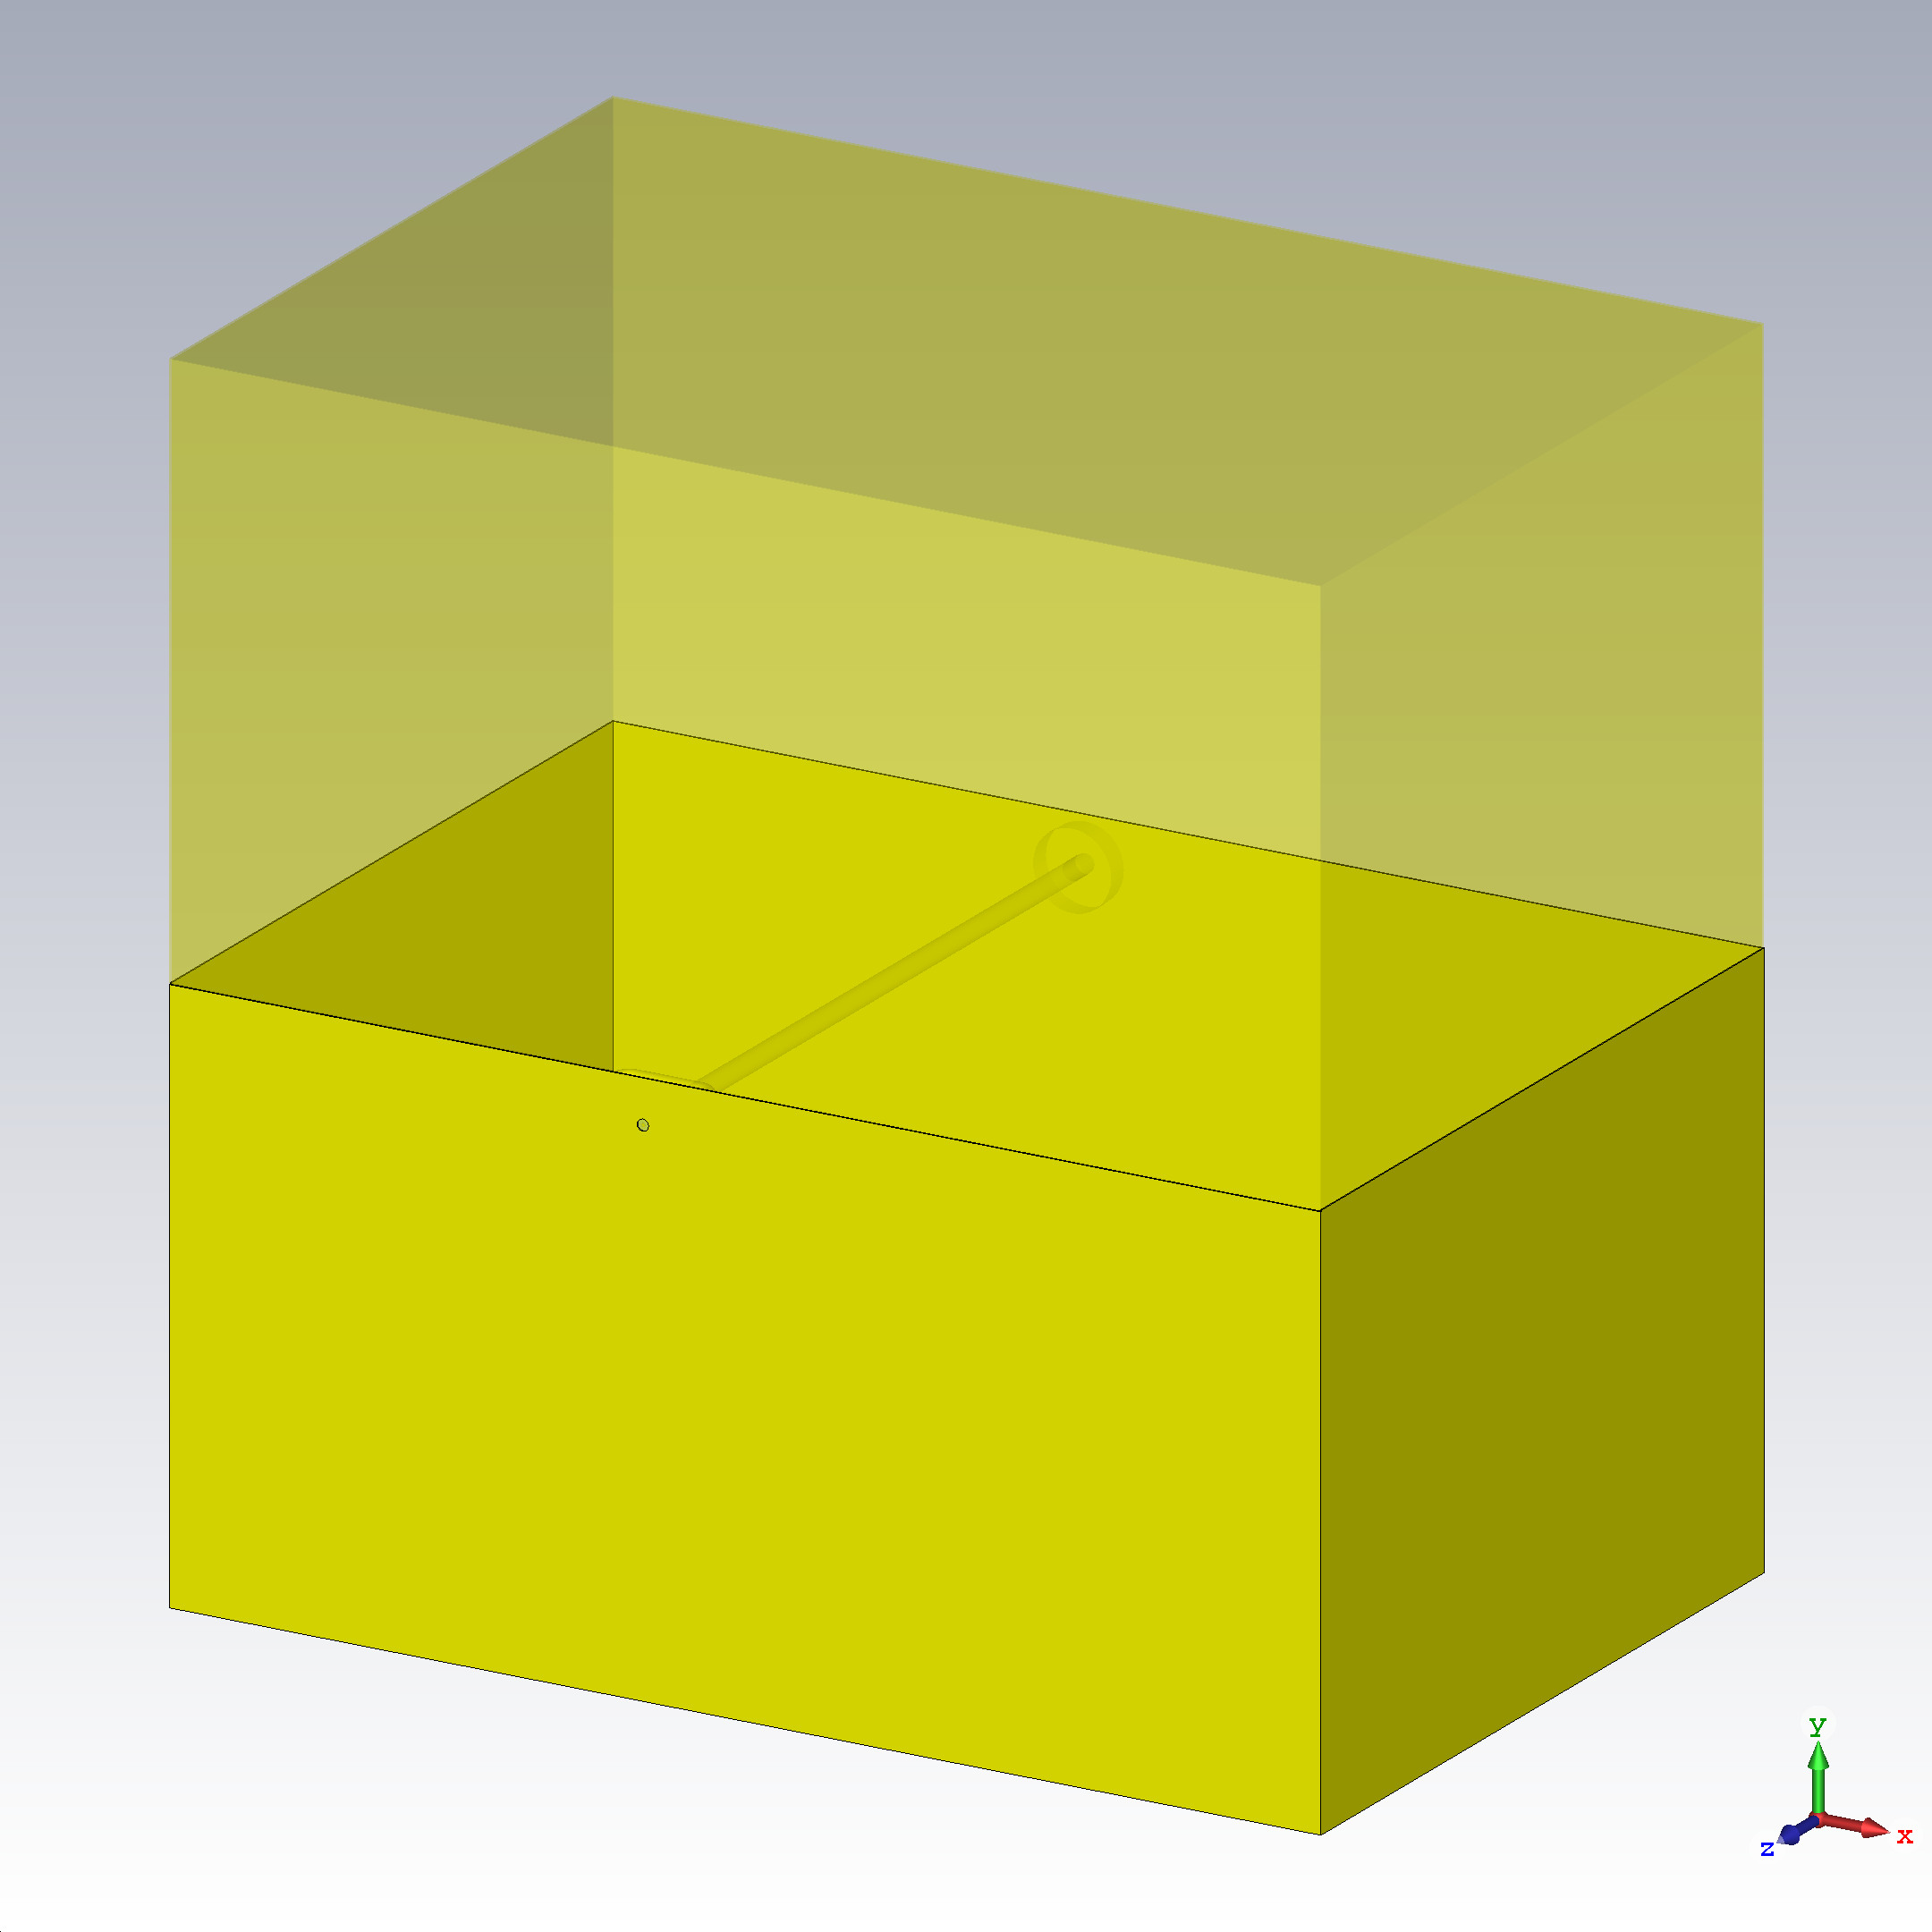
\includegraphics[height=0.4\textwidth]{./Simulation/BoxWaende2.png}
                \caption{Modell der Testbox in CST}
                \label{fig:BoxCST}
            \end{figure}
        In Abbildung~\ref{fig:InnenleiterCST} ist die Signaleinkopplung der Testbox zu sehen.
        Diese ist als Hohlzylinder aus Kupfer modelliert und geometrisch genau am realen Vorbild orientiert. Die Stange ist an der hinteren Wand elektrisch mit der Box verbunden und an der Vorderseite durch einen elektrisch nicht leitfähigen Ring aus Polyethylen (PE, CST Datenbank) von der Box isoliert. Hierdurch wird erreicht, dass die Stange als Hin- und die Boxaußenwände als Rückleiter für Signale dienen. Der Übergang zwischen Testbox, PE und Stange ist planar ausgeführt, um einen Signalport für die Simulation darzustellen.
        
            \begin{figure}[htb]
                \centering
                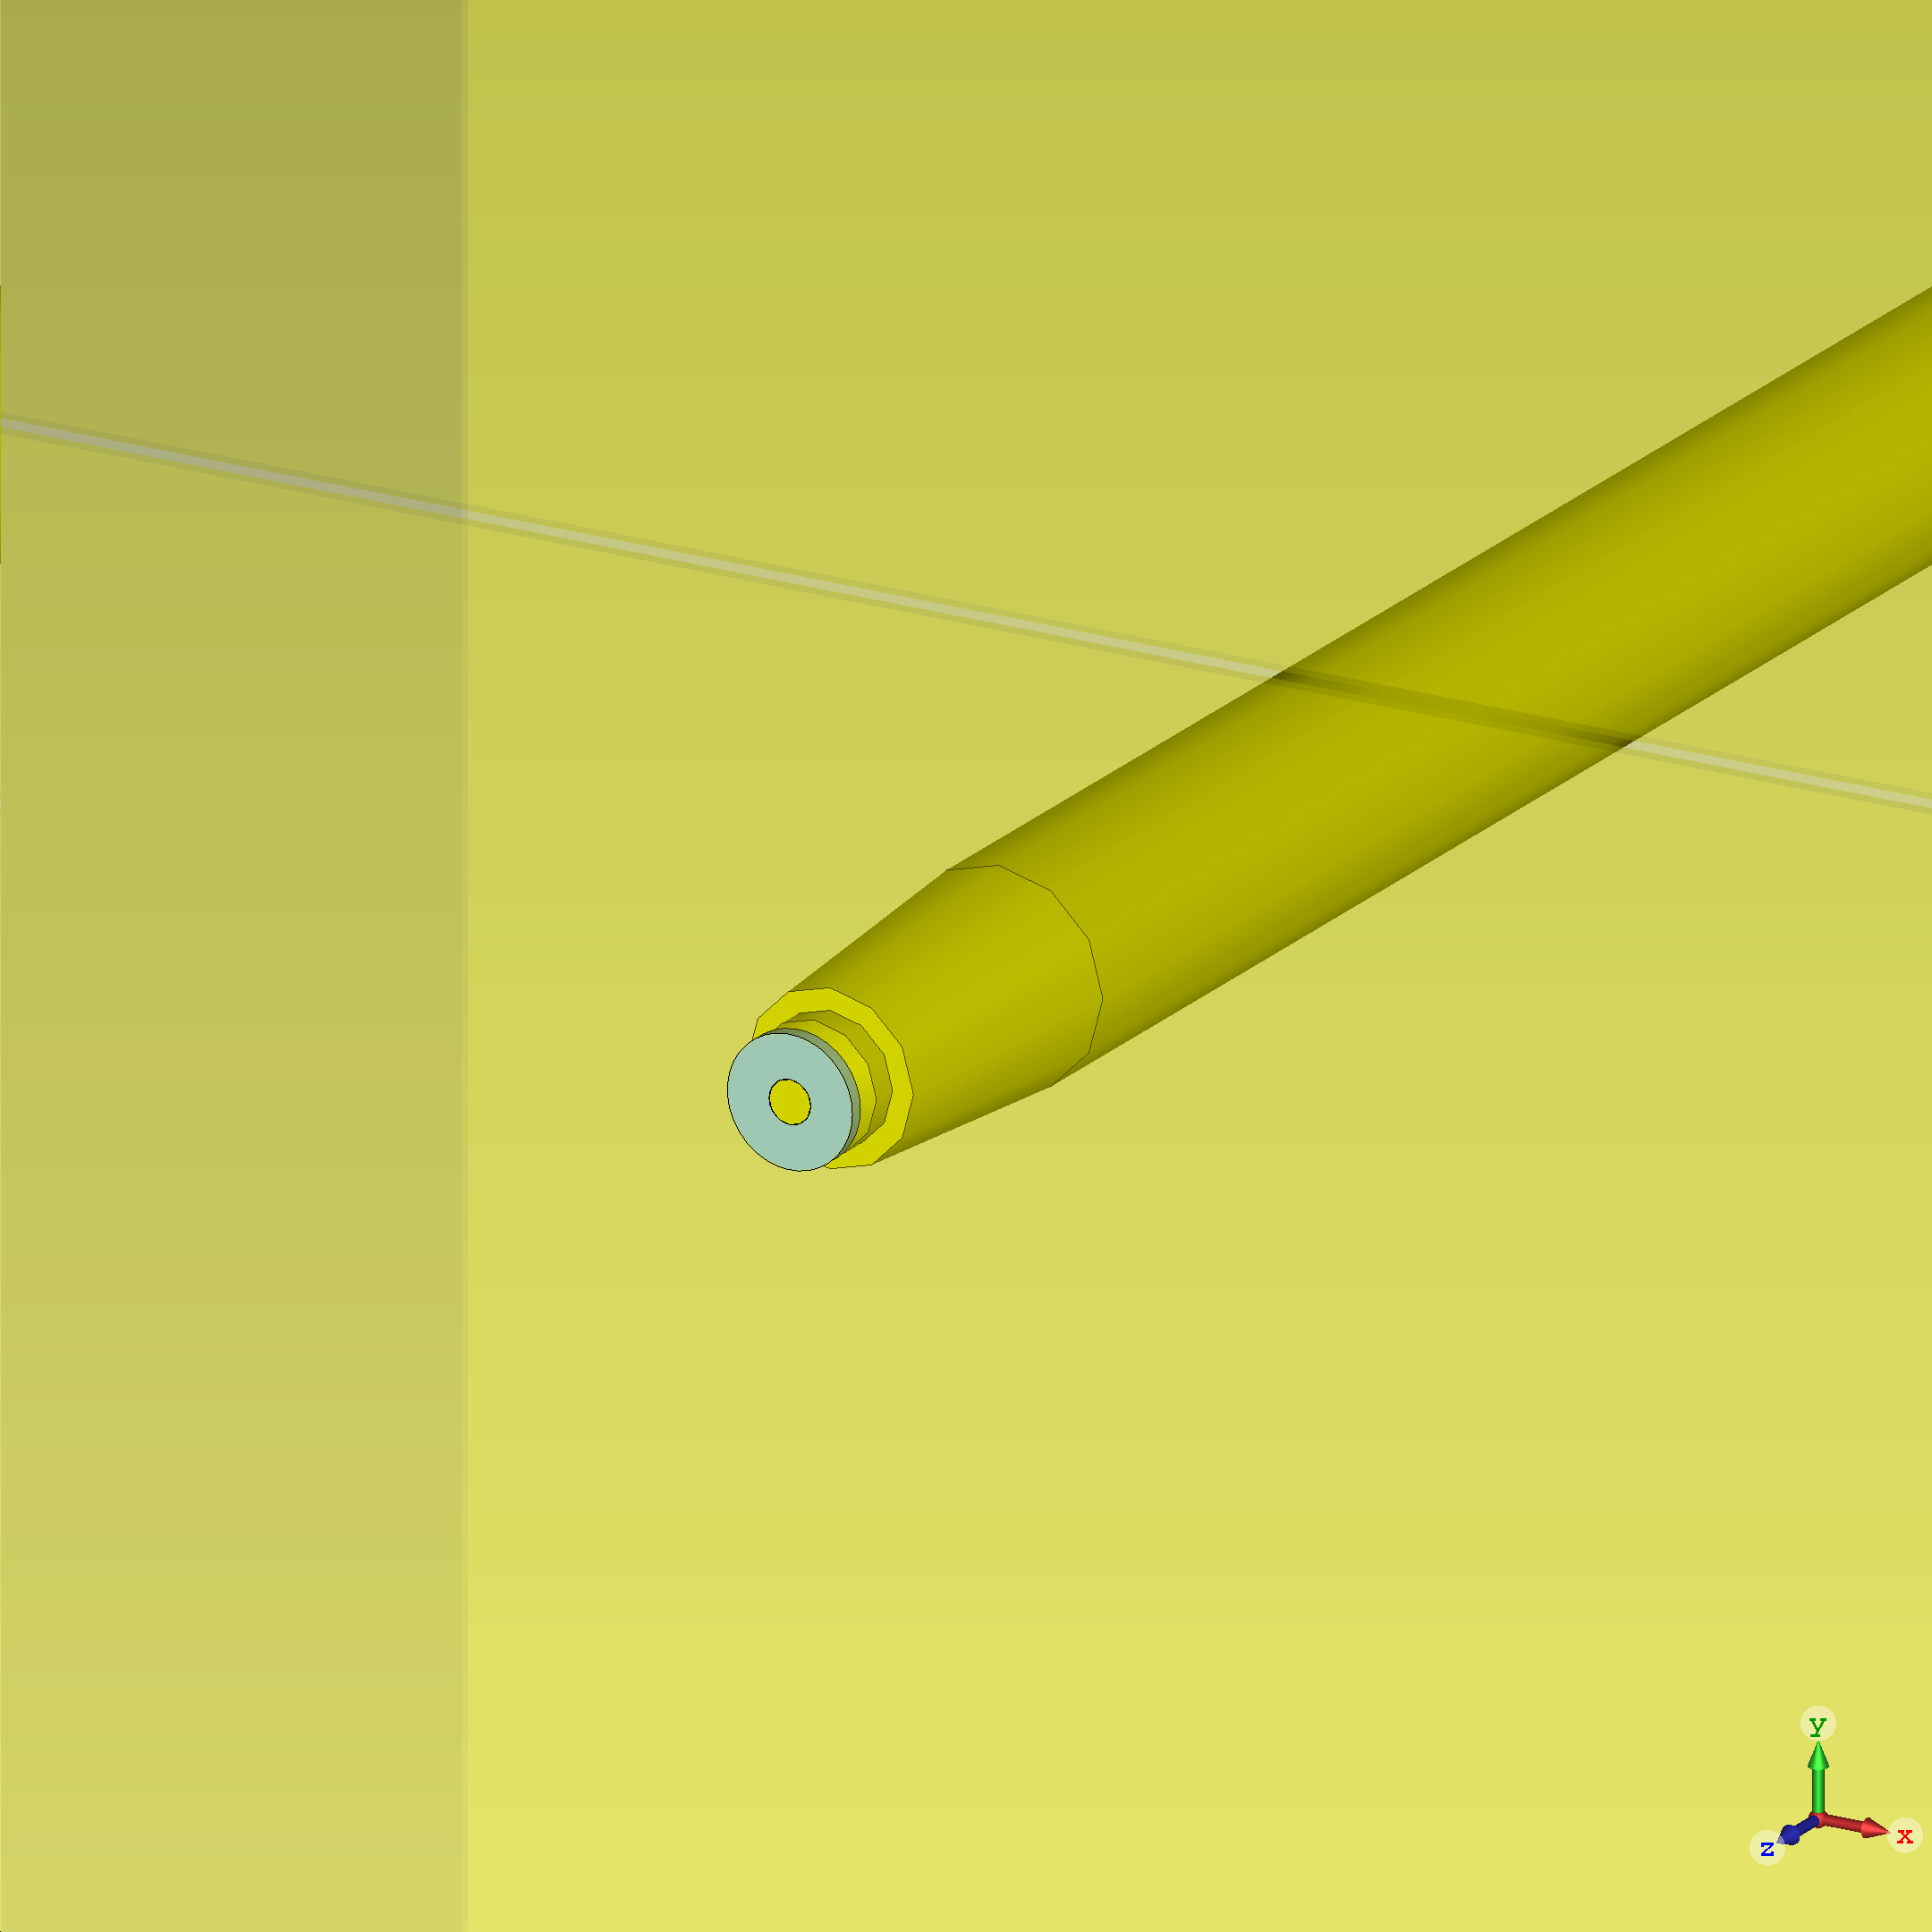
\includegraphics[height=0.4\textwidth]{./Simulation/InnenleiterPE.png}
                \caption{Modell der Einkopplungsstange mit elektrischer Isolation}
                \label{fig:InnenleiterCST}
            \end{figure}
        
        Der Ringkern ist als einfacher Hohlzylinder mit den geometrischen Abmessungen seines realen Vorbild modelliert. Dem realen Aufbau entsprechend ist er zentral im Testboxmodell, allerdings freischwebend, ohne die hölzerne Halterung, modelliert.\\
        Ein grundlegender Aspekt der Arbeit von Denys Bast~\citep{bast2017ba} ist, die magnetische Permeabilität des Ringkernmaterials in der Simulation mit dem realen Material in Übereinstimmung zu bringen. Die dabei gewonnenen Daten wurden übernommen.
        
            \begin{figure}[htb]
                \centering
                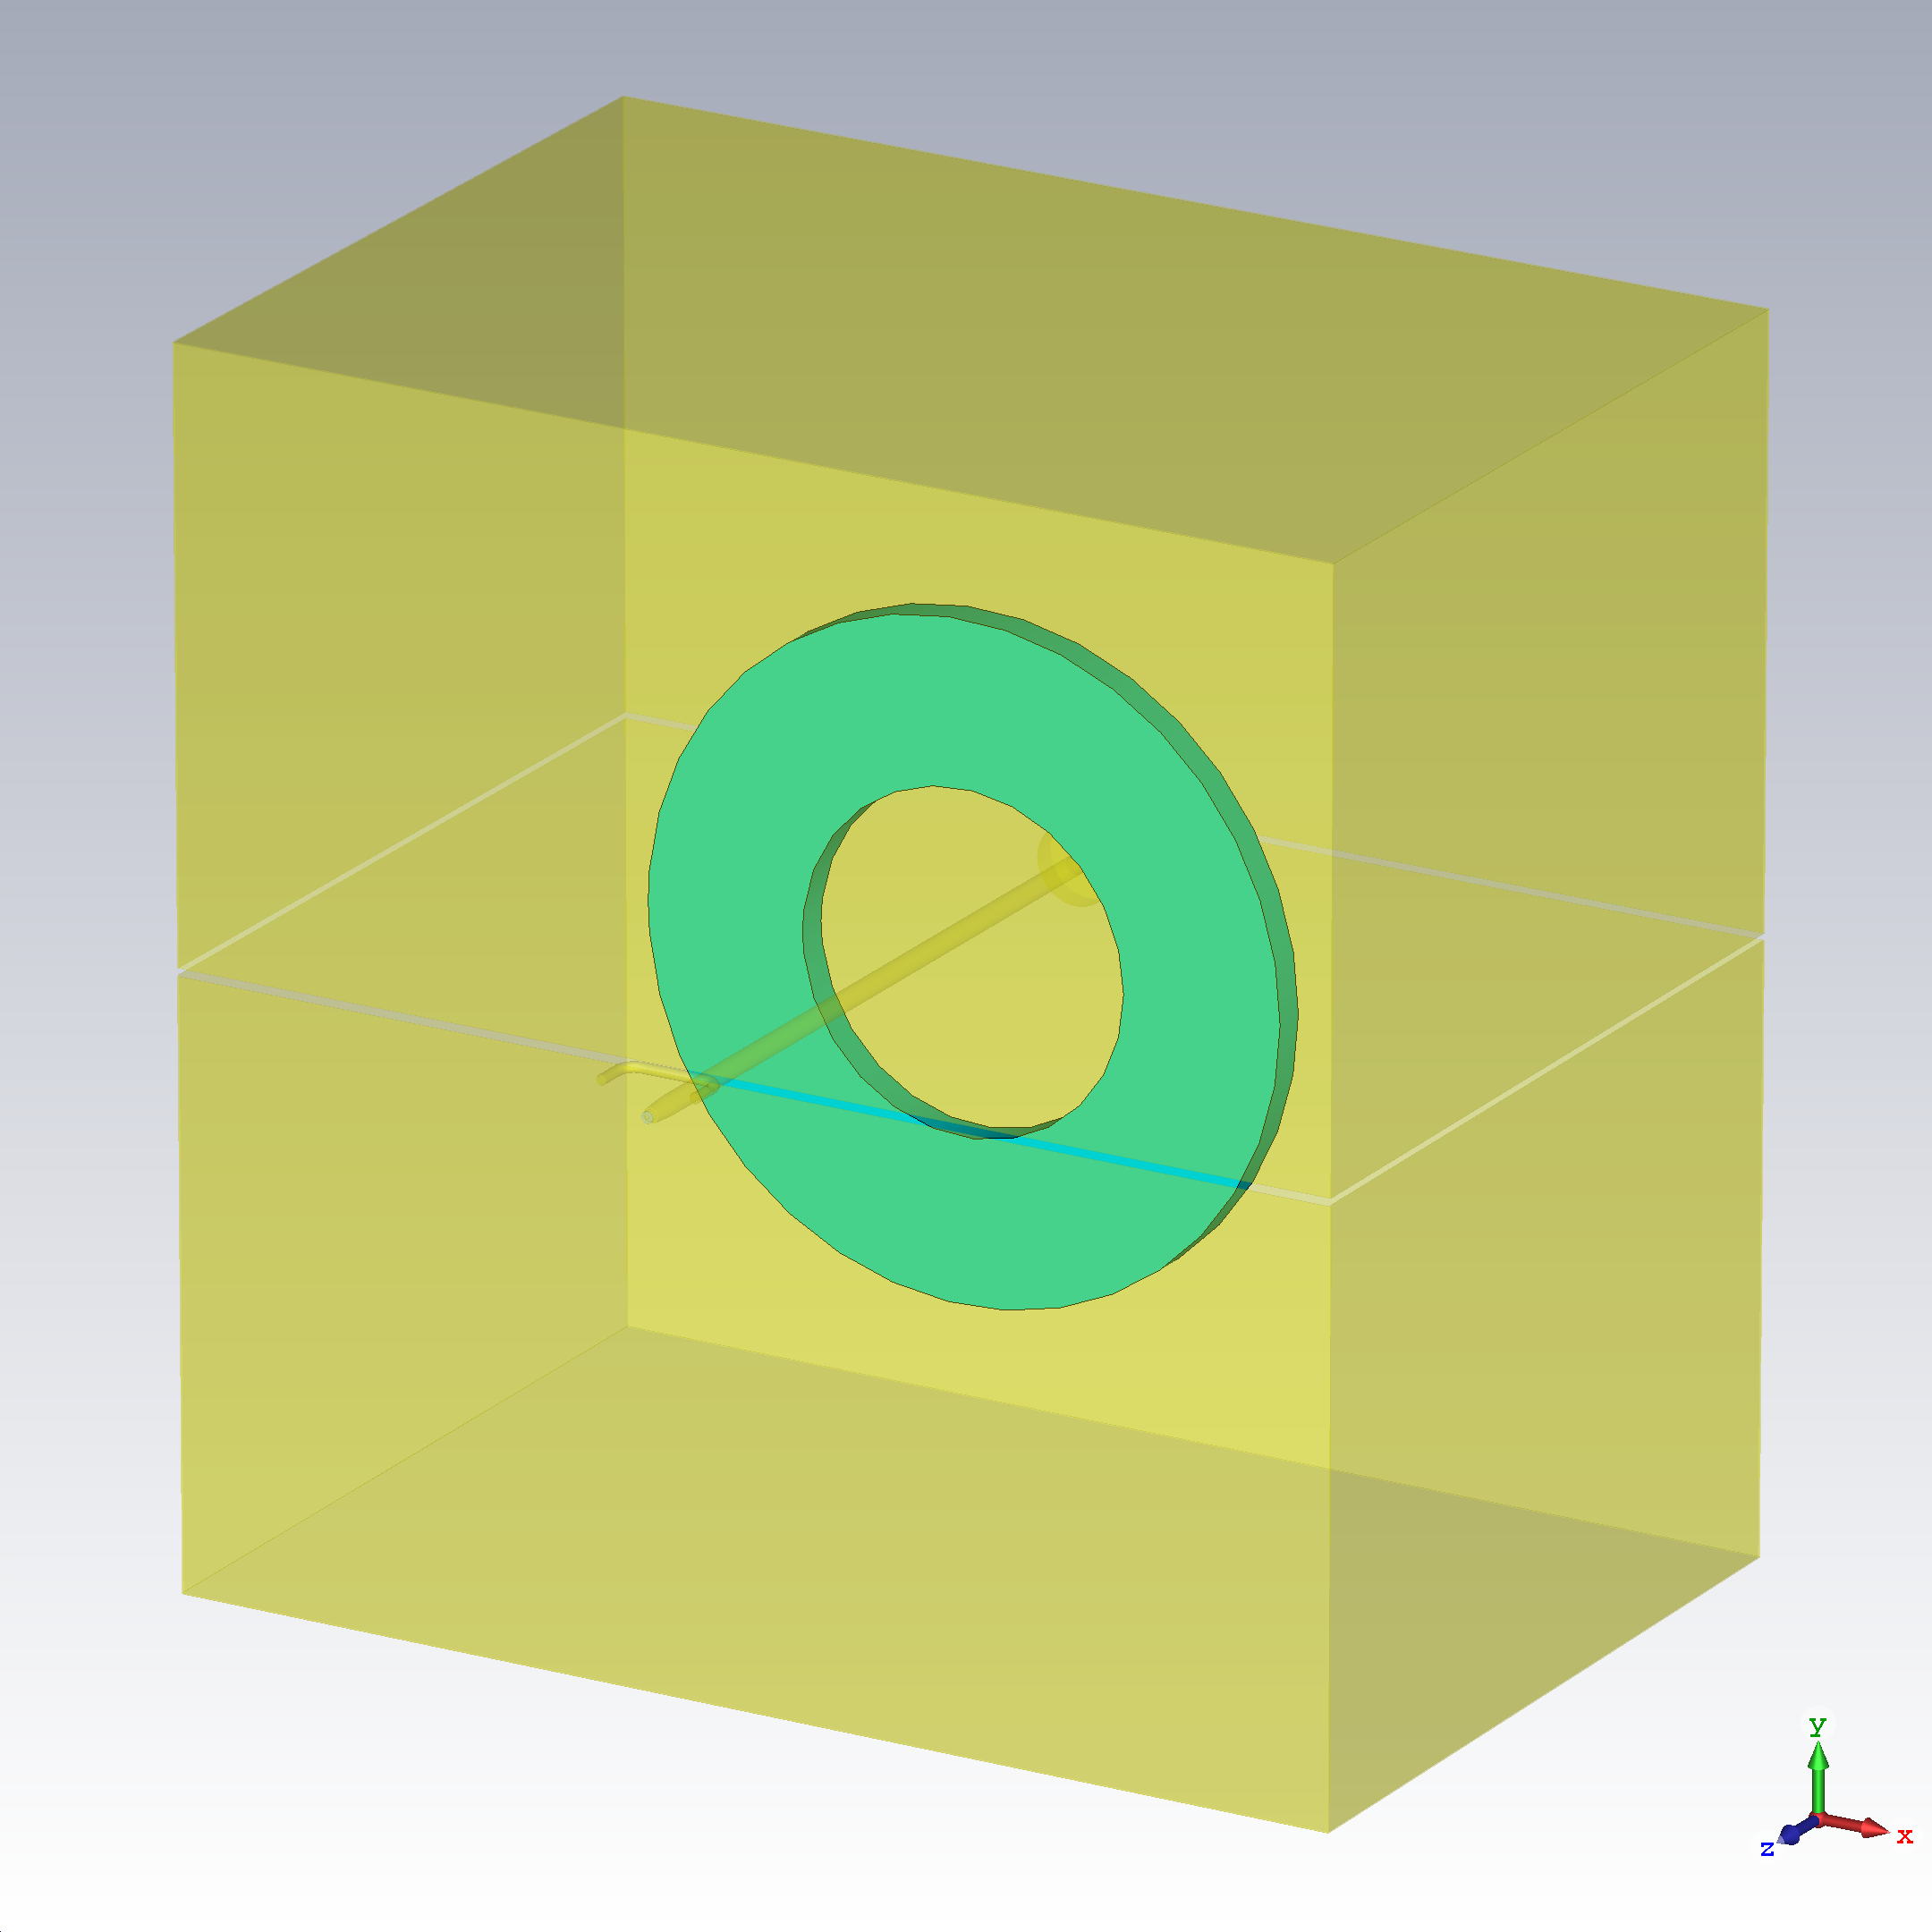
\includegraphics[height=0.4\textwidth]{./Simulation/BoxRK.png}
                \caption{Gesamtdarstellung der Modellierung von Testbox und Ringkern nach Denys Bast~\citep{bast2017ba}}
                \label{fig:BoxRKCST}
            \end{figure}
        
        Abbildung~\ref{fig:BoxRKCST} bildet den modellierten Aufbau der Testbox mit Ringkern ab, wie er in \citep{bast2017ba} beschrieben wird.

        \subsection{Kurzschlüsse}
        Die für die Parameteranalyse dieser Arbeit benötigten Kurzschlüsse sind in CST in verschiedenen, komplexen Ausführungen modelliert.\\
        Die erste Version stellt ein einfacher, ellipsenförmiger Torus dar, wie er in Abbildung~\ref{fig:KSCST}\subref{subfig:V1} abgebildet ist. Als Material für die Simulation wird Kupfer aus der Datenbank von CST verwendet.\\
        Die in Kapitel~\ref{sec:testbox} beschriebenen Verbesserungen der Kurzschlüsse für eine erhöhte Reproduzierbarkeit der Messungen, sind so in CST modelliert. Abbildung~\ref{fig:KSCST}\subref{subfig:V2} zeigt die Umformung des einfachen Torus zu einem schienenförmigen Kurzschluss. Die finale Version, die letztlich für die Messungen benutzt wurde, ist in Abbildung~\ref{fig:KSCST}\subref{subfig:V3} zu sehen. Die einfache Kupferschiene ist geometrisch an die verwendeten Kurzschlüsse angepasst und um die Verbindungsschrauben erweitert.
        
            \begin{figure}[htb]
                \centering
                \subfloat[Version 1]{
                    \label{subfig:V1}
                    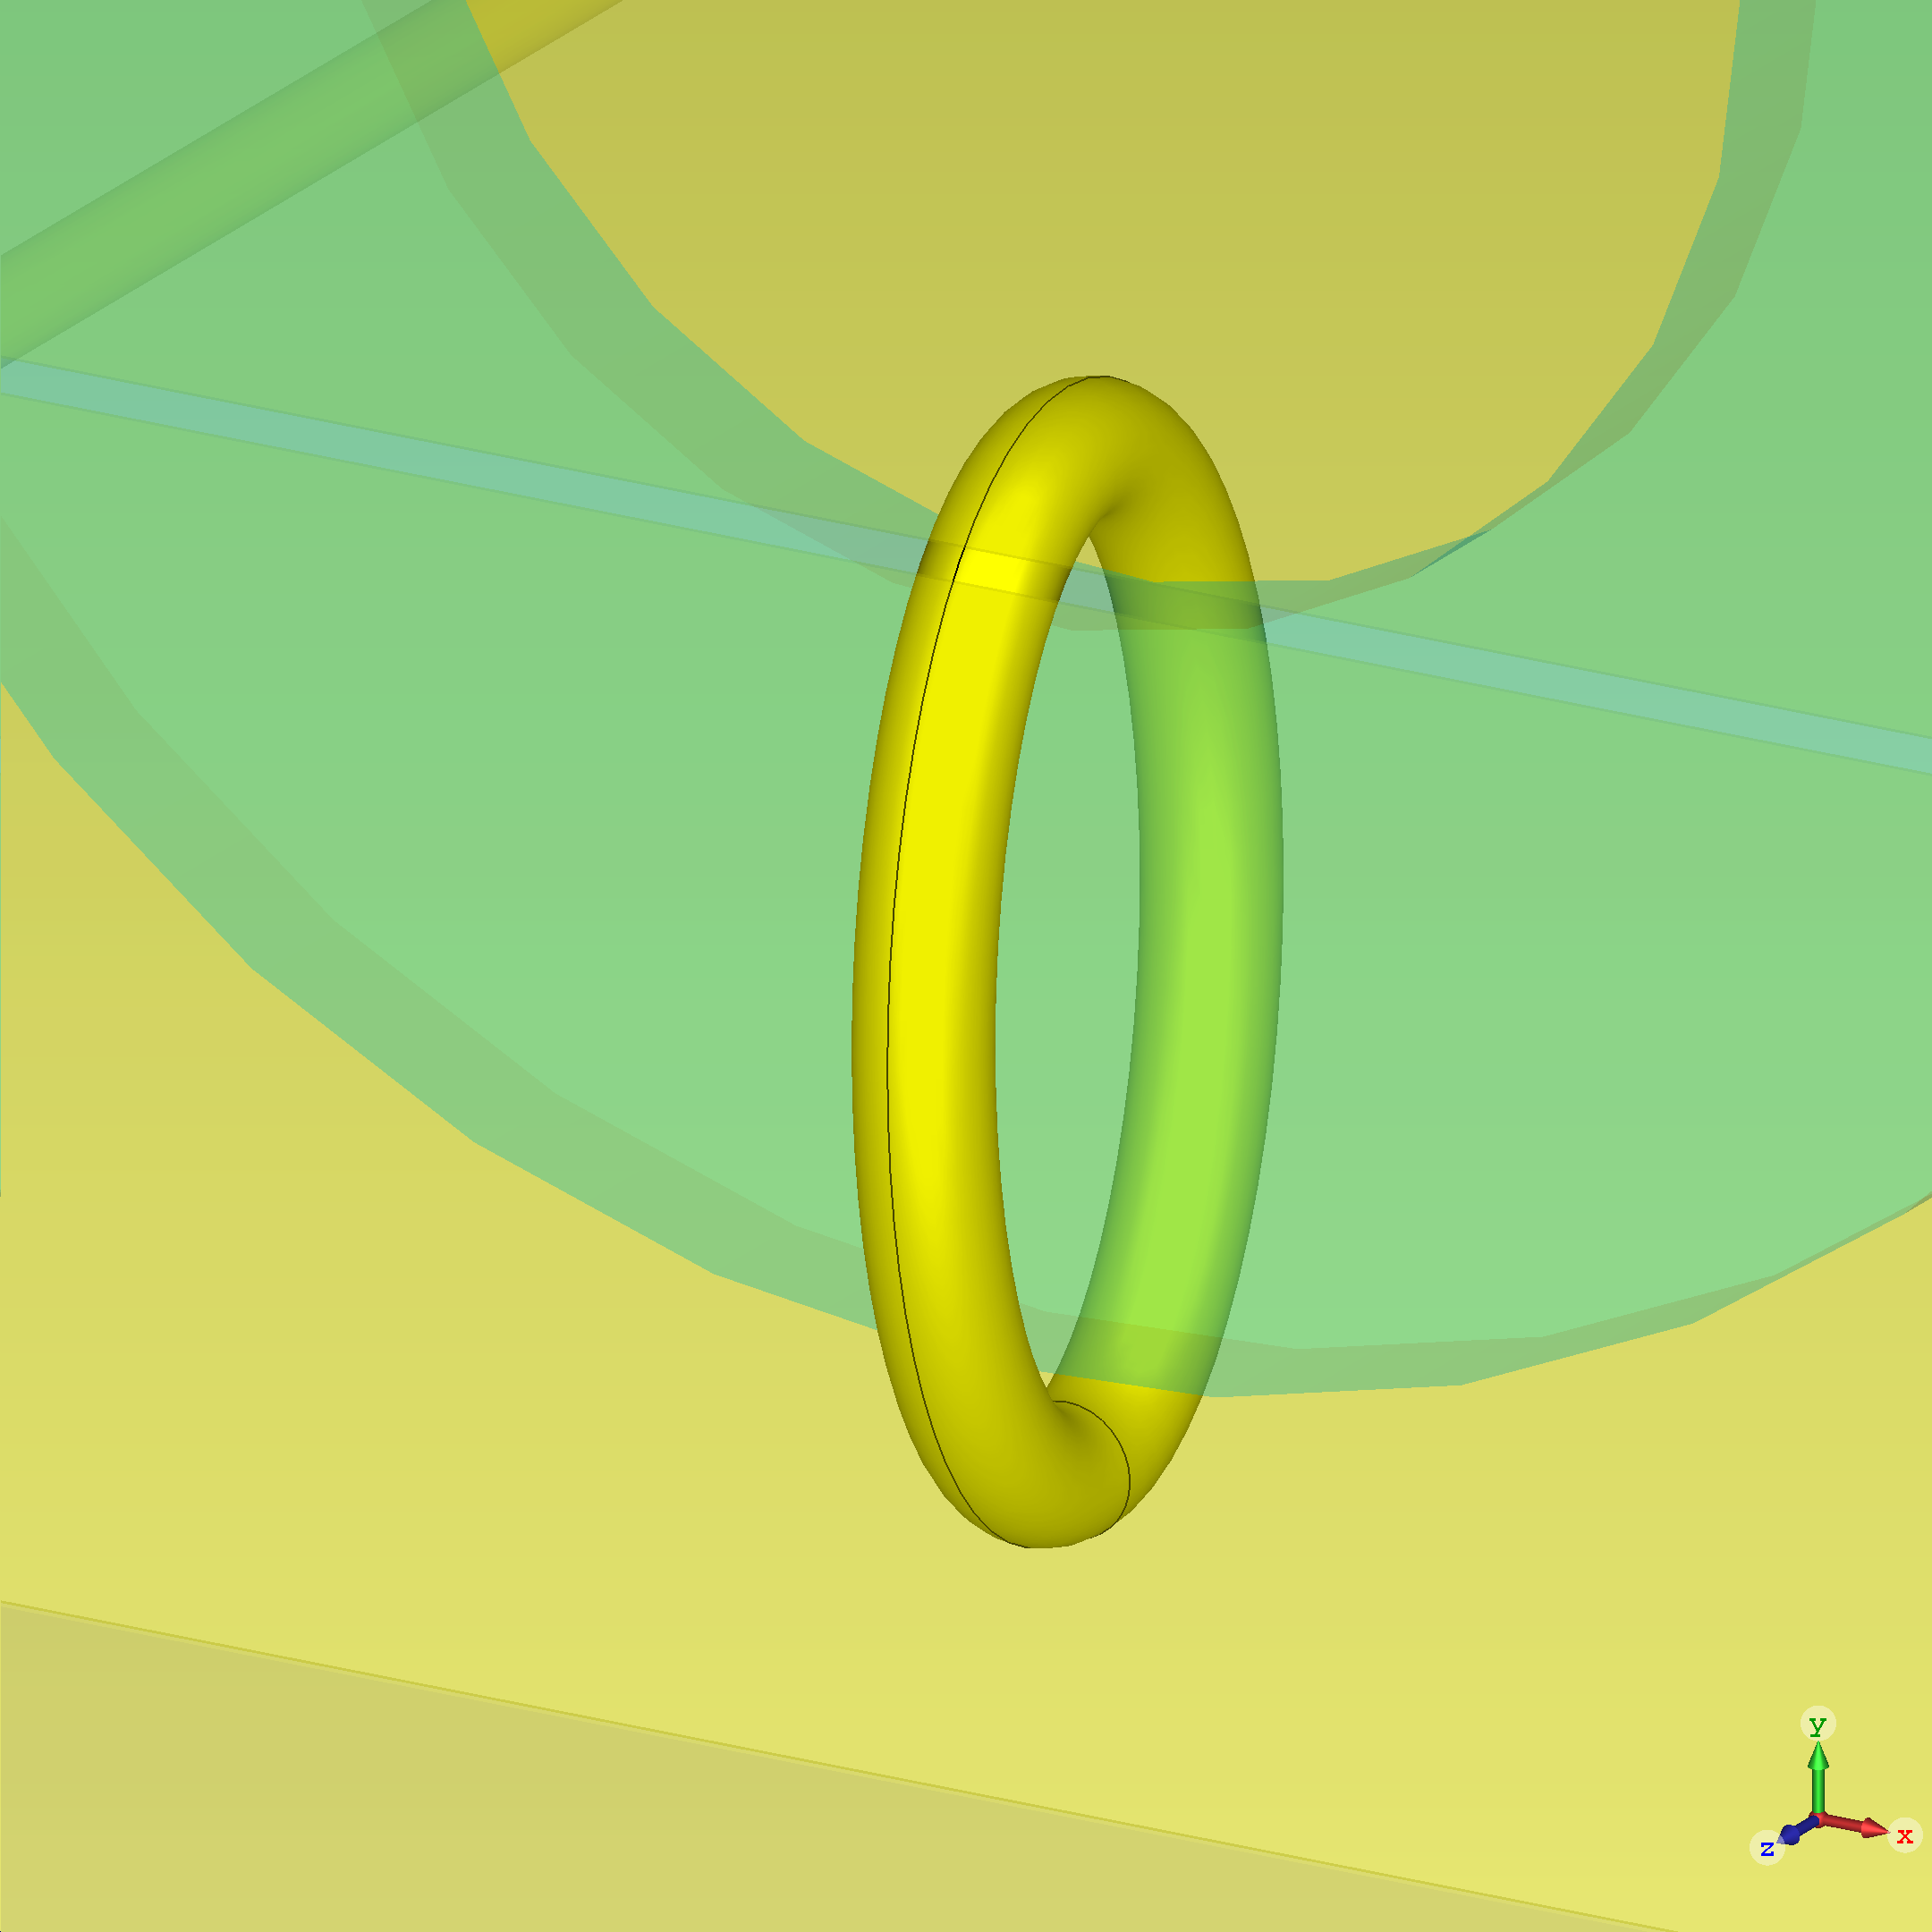
\includegraphics[height=0.3\textwidth]{./Simulation/KSV1Torus.png}}
                \hspace{0.01\textwidth}
                \subfloat[Version 2]{
                    \label{subfig:V2}
                    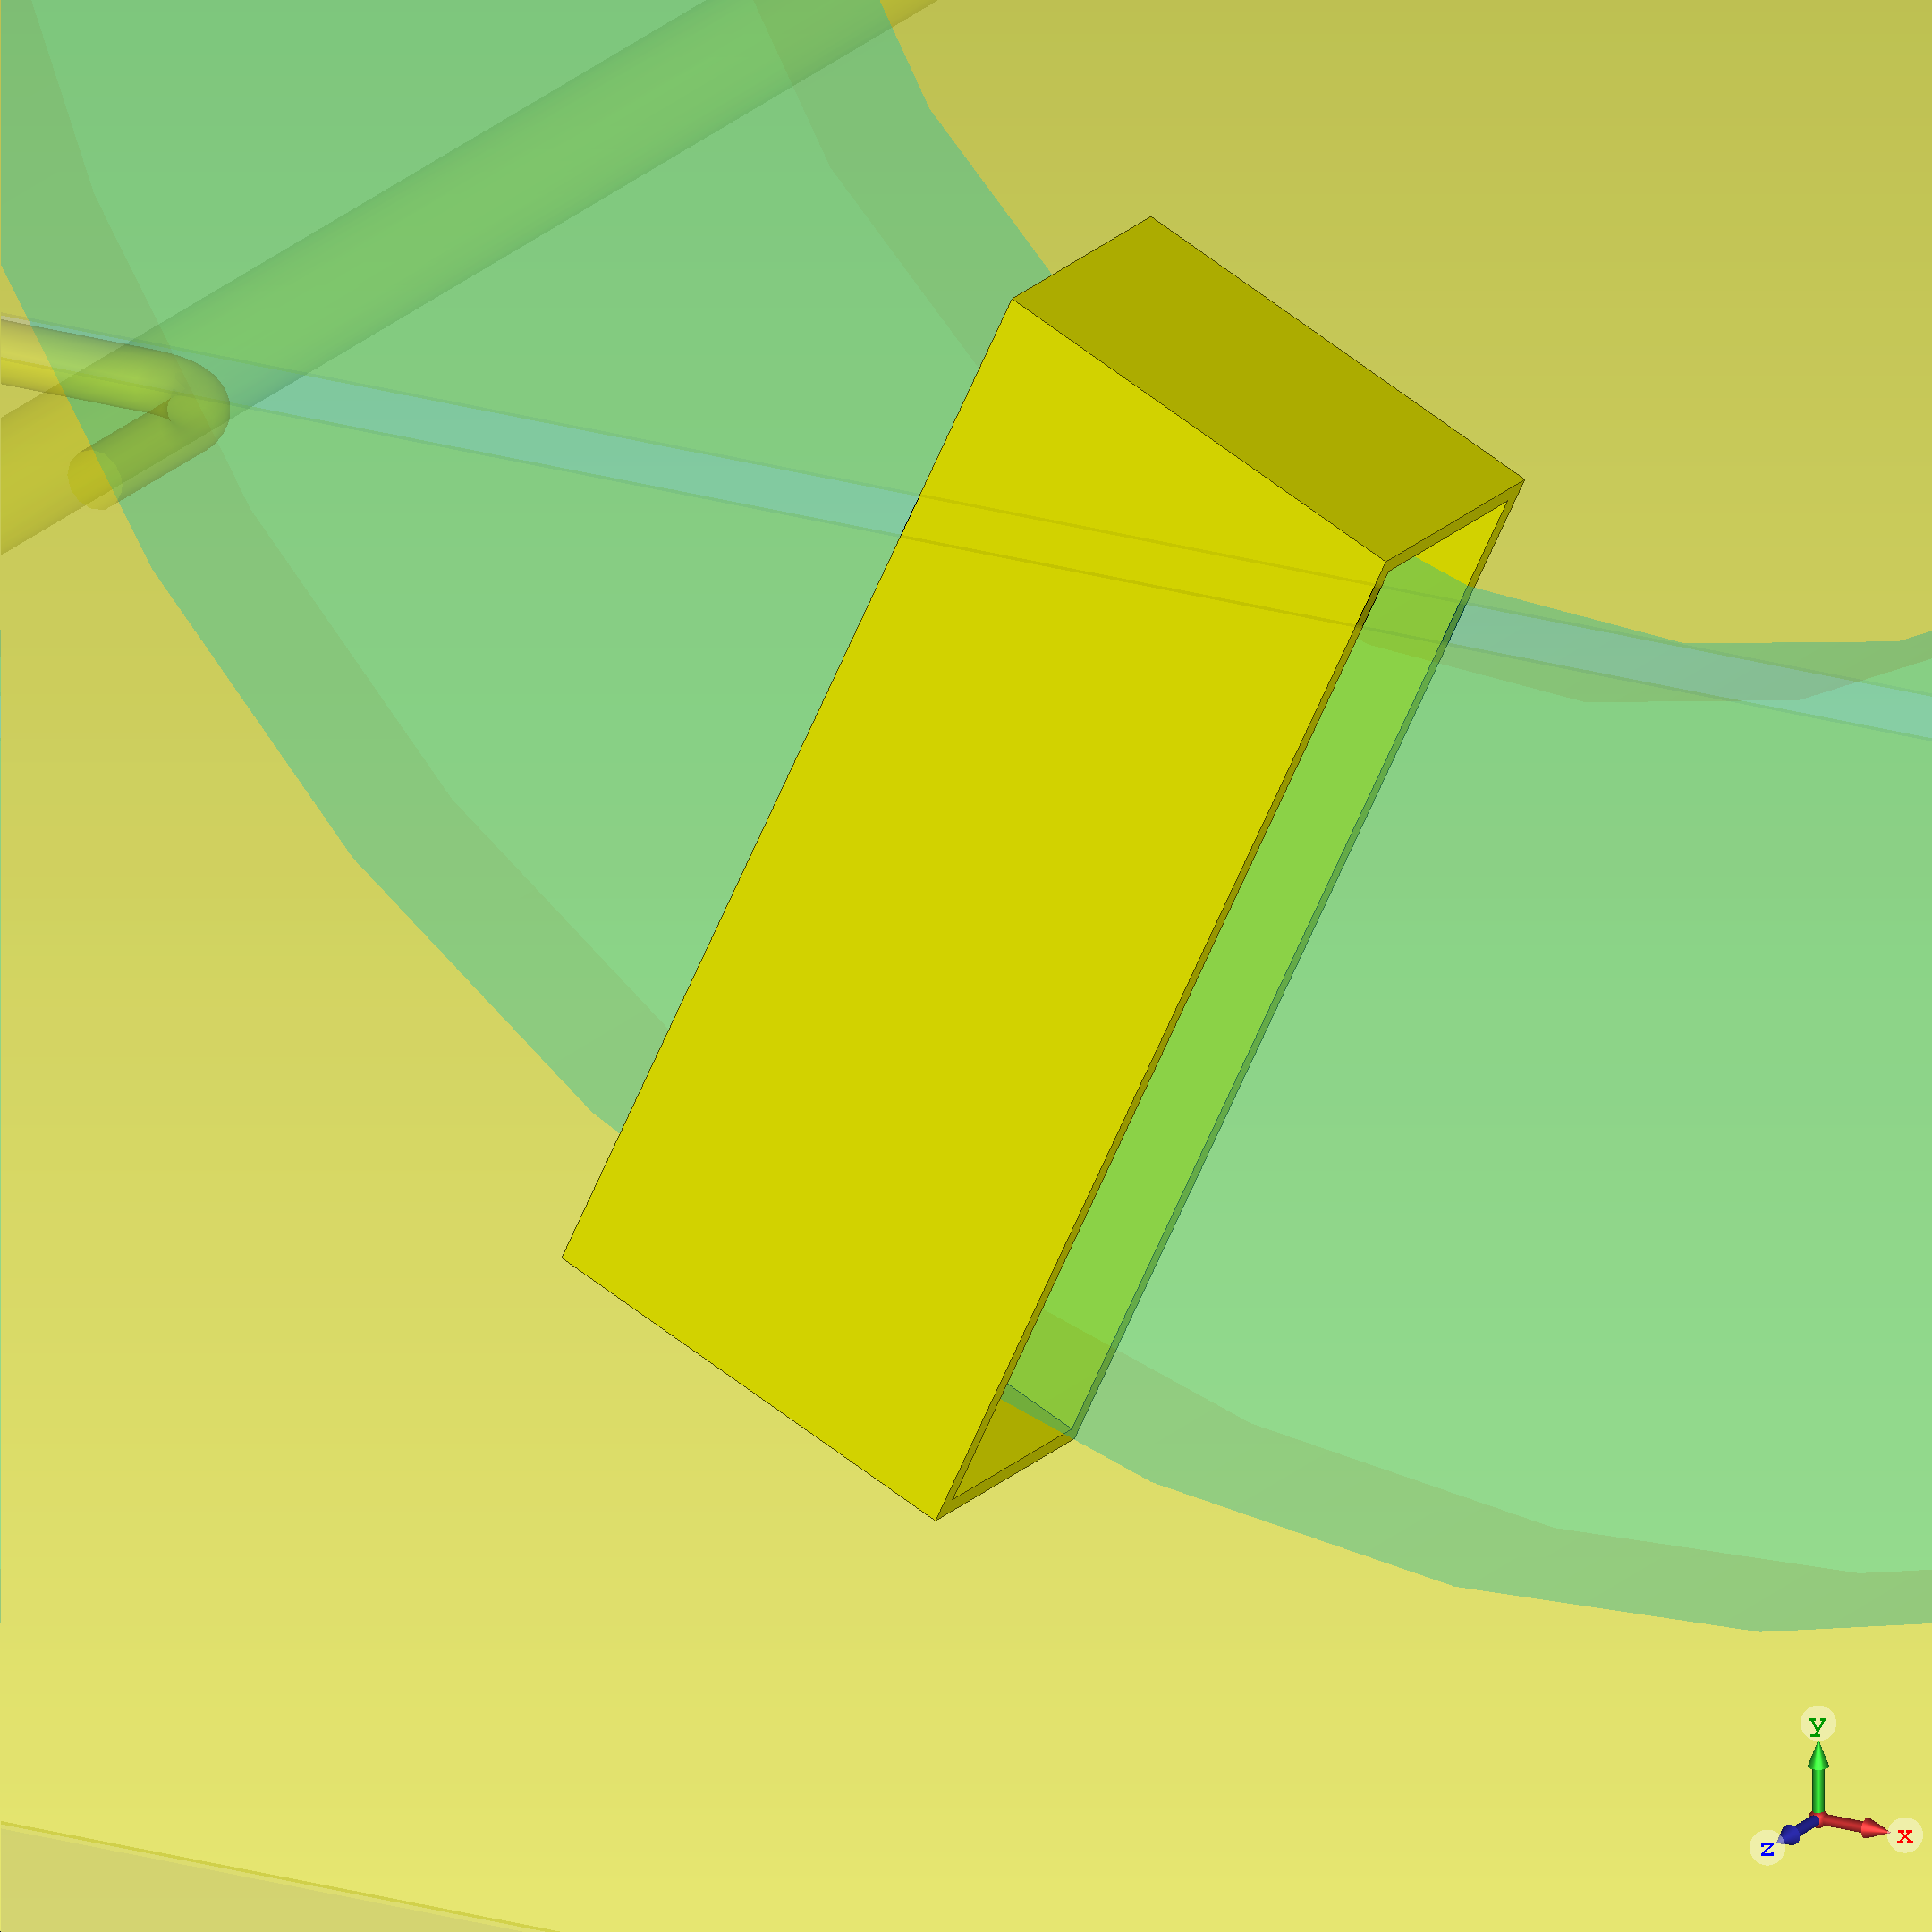
\includegraphics[height=0.3\textwidth]{./Simulation/KSV2Schiene.png}}
                \hspace{0.01\textwidth}
                \subfloat[Version 3]{
                    \label{subfig:V3}
                    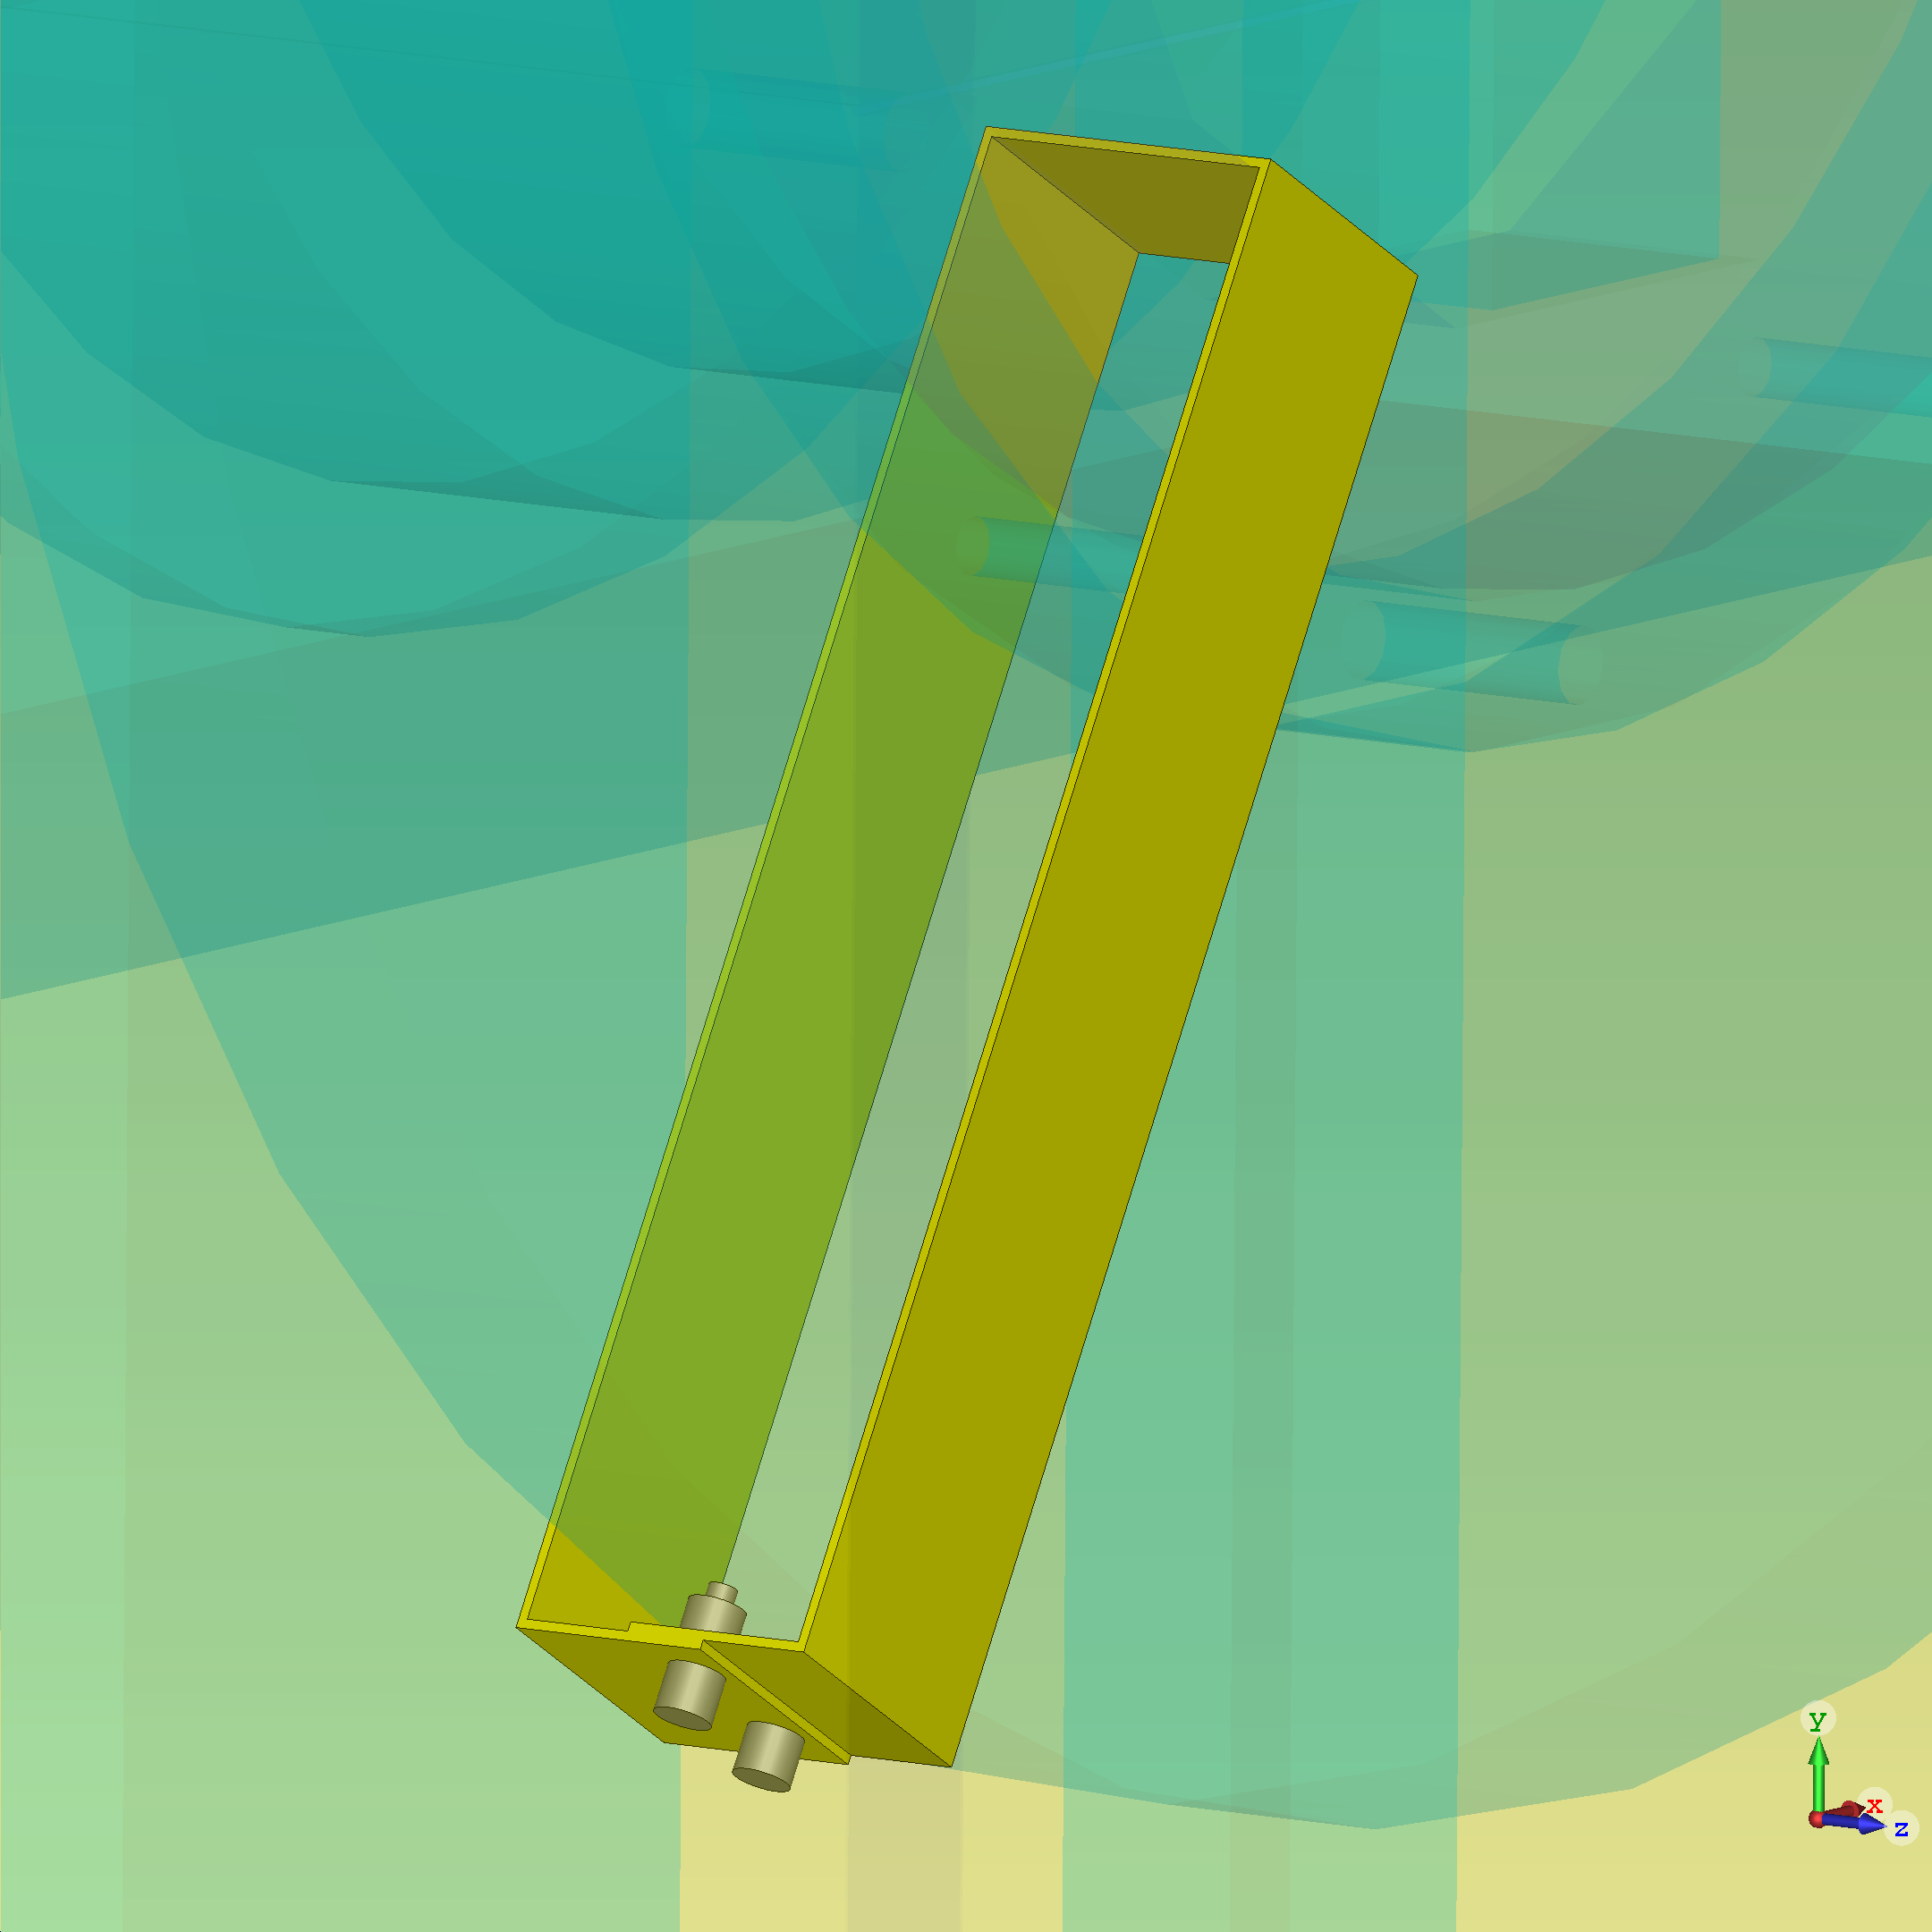
\includegraphics[height=0.3\textwidth]{./Simulation/KSV3MitSchrauben.png}}
                \caption{Modellierung eines Kurzschluss \protect\subref{subfig:V1} als Torus, \protect\subref{subfig:V2} als Schiene und \protect\subref{subfig:V3} in gefertigter Ausführung.}
                \label{fig:KSCST}
            \end{figure}
        
        Um eine Parameteranalyse durchzuführen und die Simulationsergebnisse mit den Messungen gegenüberzustellen, ist die finale Version in den verschiedenen Ausführungen, wie sie aus Kapitel~\ref{sec:shorts} hervorgehen, nachgebildet.
        
        \subsection{Realitätsgetreue Anpassungen}
        Das bestehende Modell wurde im Laufe der Arbeit weiter ausarbeitet, um die Übereinstimmung der Simulationsergebnisse mit den Messungen zu erhöhen. Die nachfolgenden Komponenten wurden in das CST-Modell übernommen, da aufgrund ihrer di-/elektrischen Eigenschaften ein Einfluss auf die Simulation zu erwarten ist.\\
        \todo[inline,color=red!30]{$\uparrow$ Verweis auf Simulationsergebnisse, wenn Kapitel vorhanden. $\uparrow$}
        Wie auf den Bildern der Testbox in Kapitel~\ref{chap:messaufbau} hervorgeht, befindet sich oberhalb der Einkopplungsstange an der Anschlussseite ein metallischer Bügel. Er ist möglichst exakt in CST nachgebildet (siehe Abb.~\ref{fig:AnpassungCST}\subref{subfig:Buegel}).\\
        Am Ende der Einkopplungsstange an der Rückwand ist eine zylinderförmige, kupferne Halterung für die Stange montiert, sie ist nach Abbildung~\ref{fig:AnpassungCST}\subref{subfig:Block} modelliert.
        \par
        Zuletzt wurde für diese Arbeit auch die Holzkonstruktion in CST übernommen, die als Halterung für die Ringkerne in der Testbox dient (siehe Abb.~\ref{fig:AnpassungCST}\subref{subfig:HolzKonst}). Dabei wurden die Holzkreise mit einem dissipativen, durch Austesten und die Messung Anpassen bestimmten $\underline{\varepsilon}_r(\omega) = \varepsilon_r'(\omega)-i\varepsilon_r''(\omega)$ modelliert, da es sich hierbei nicht um die Standardholzmodellierung von CST handelt, wie sie für die Holzbalken verwendet wird, sondern ein geschichtetes Pressspanholz verwendet wird.
        
            \begin{figure}[htb]
                \centering
                \subfloat[Bügel]{
                    \label{subfig:Buegel}
                    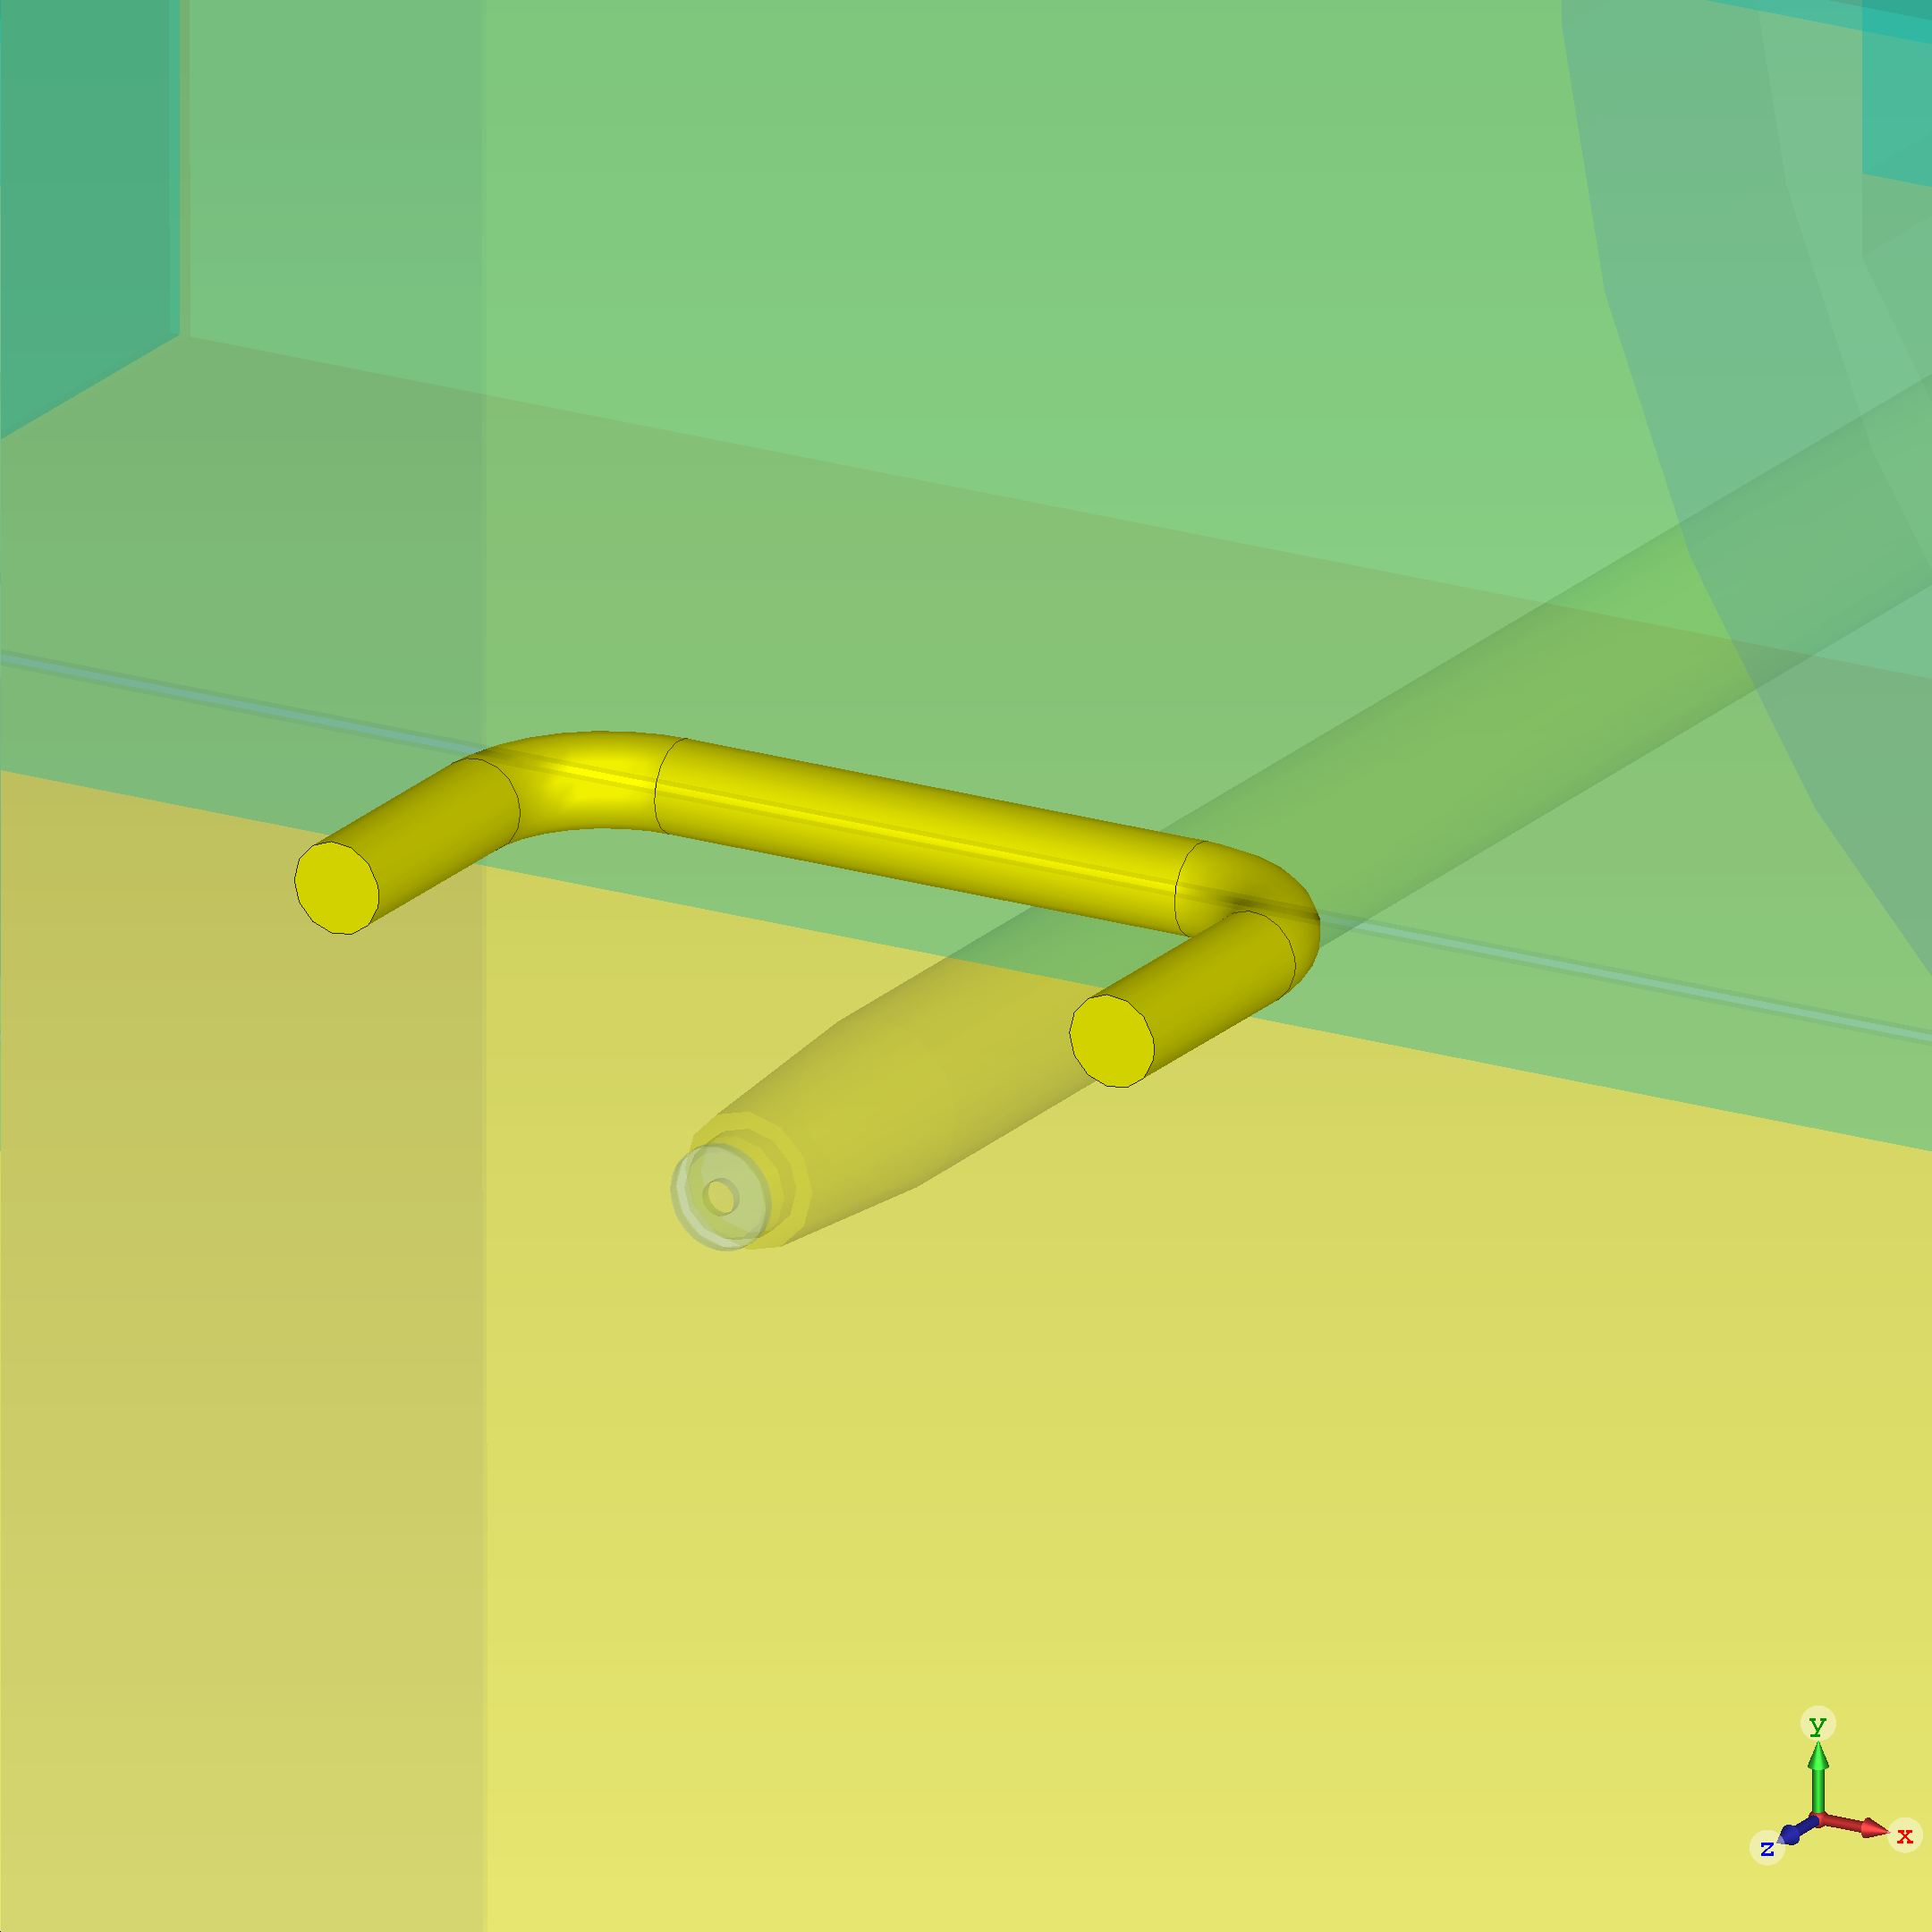
\includegraphics[height=0.3\textwidth]{./Simulation/Buegel.png}}
                \hspace{0.01\textwidth}
                \subfloat[Zylinder]{
                    \label{subfig:Block}
                    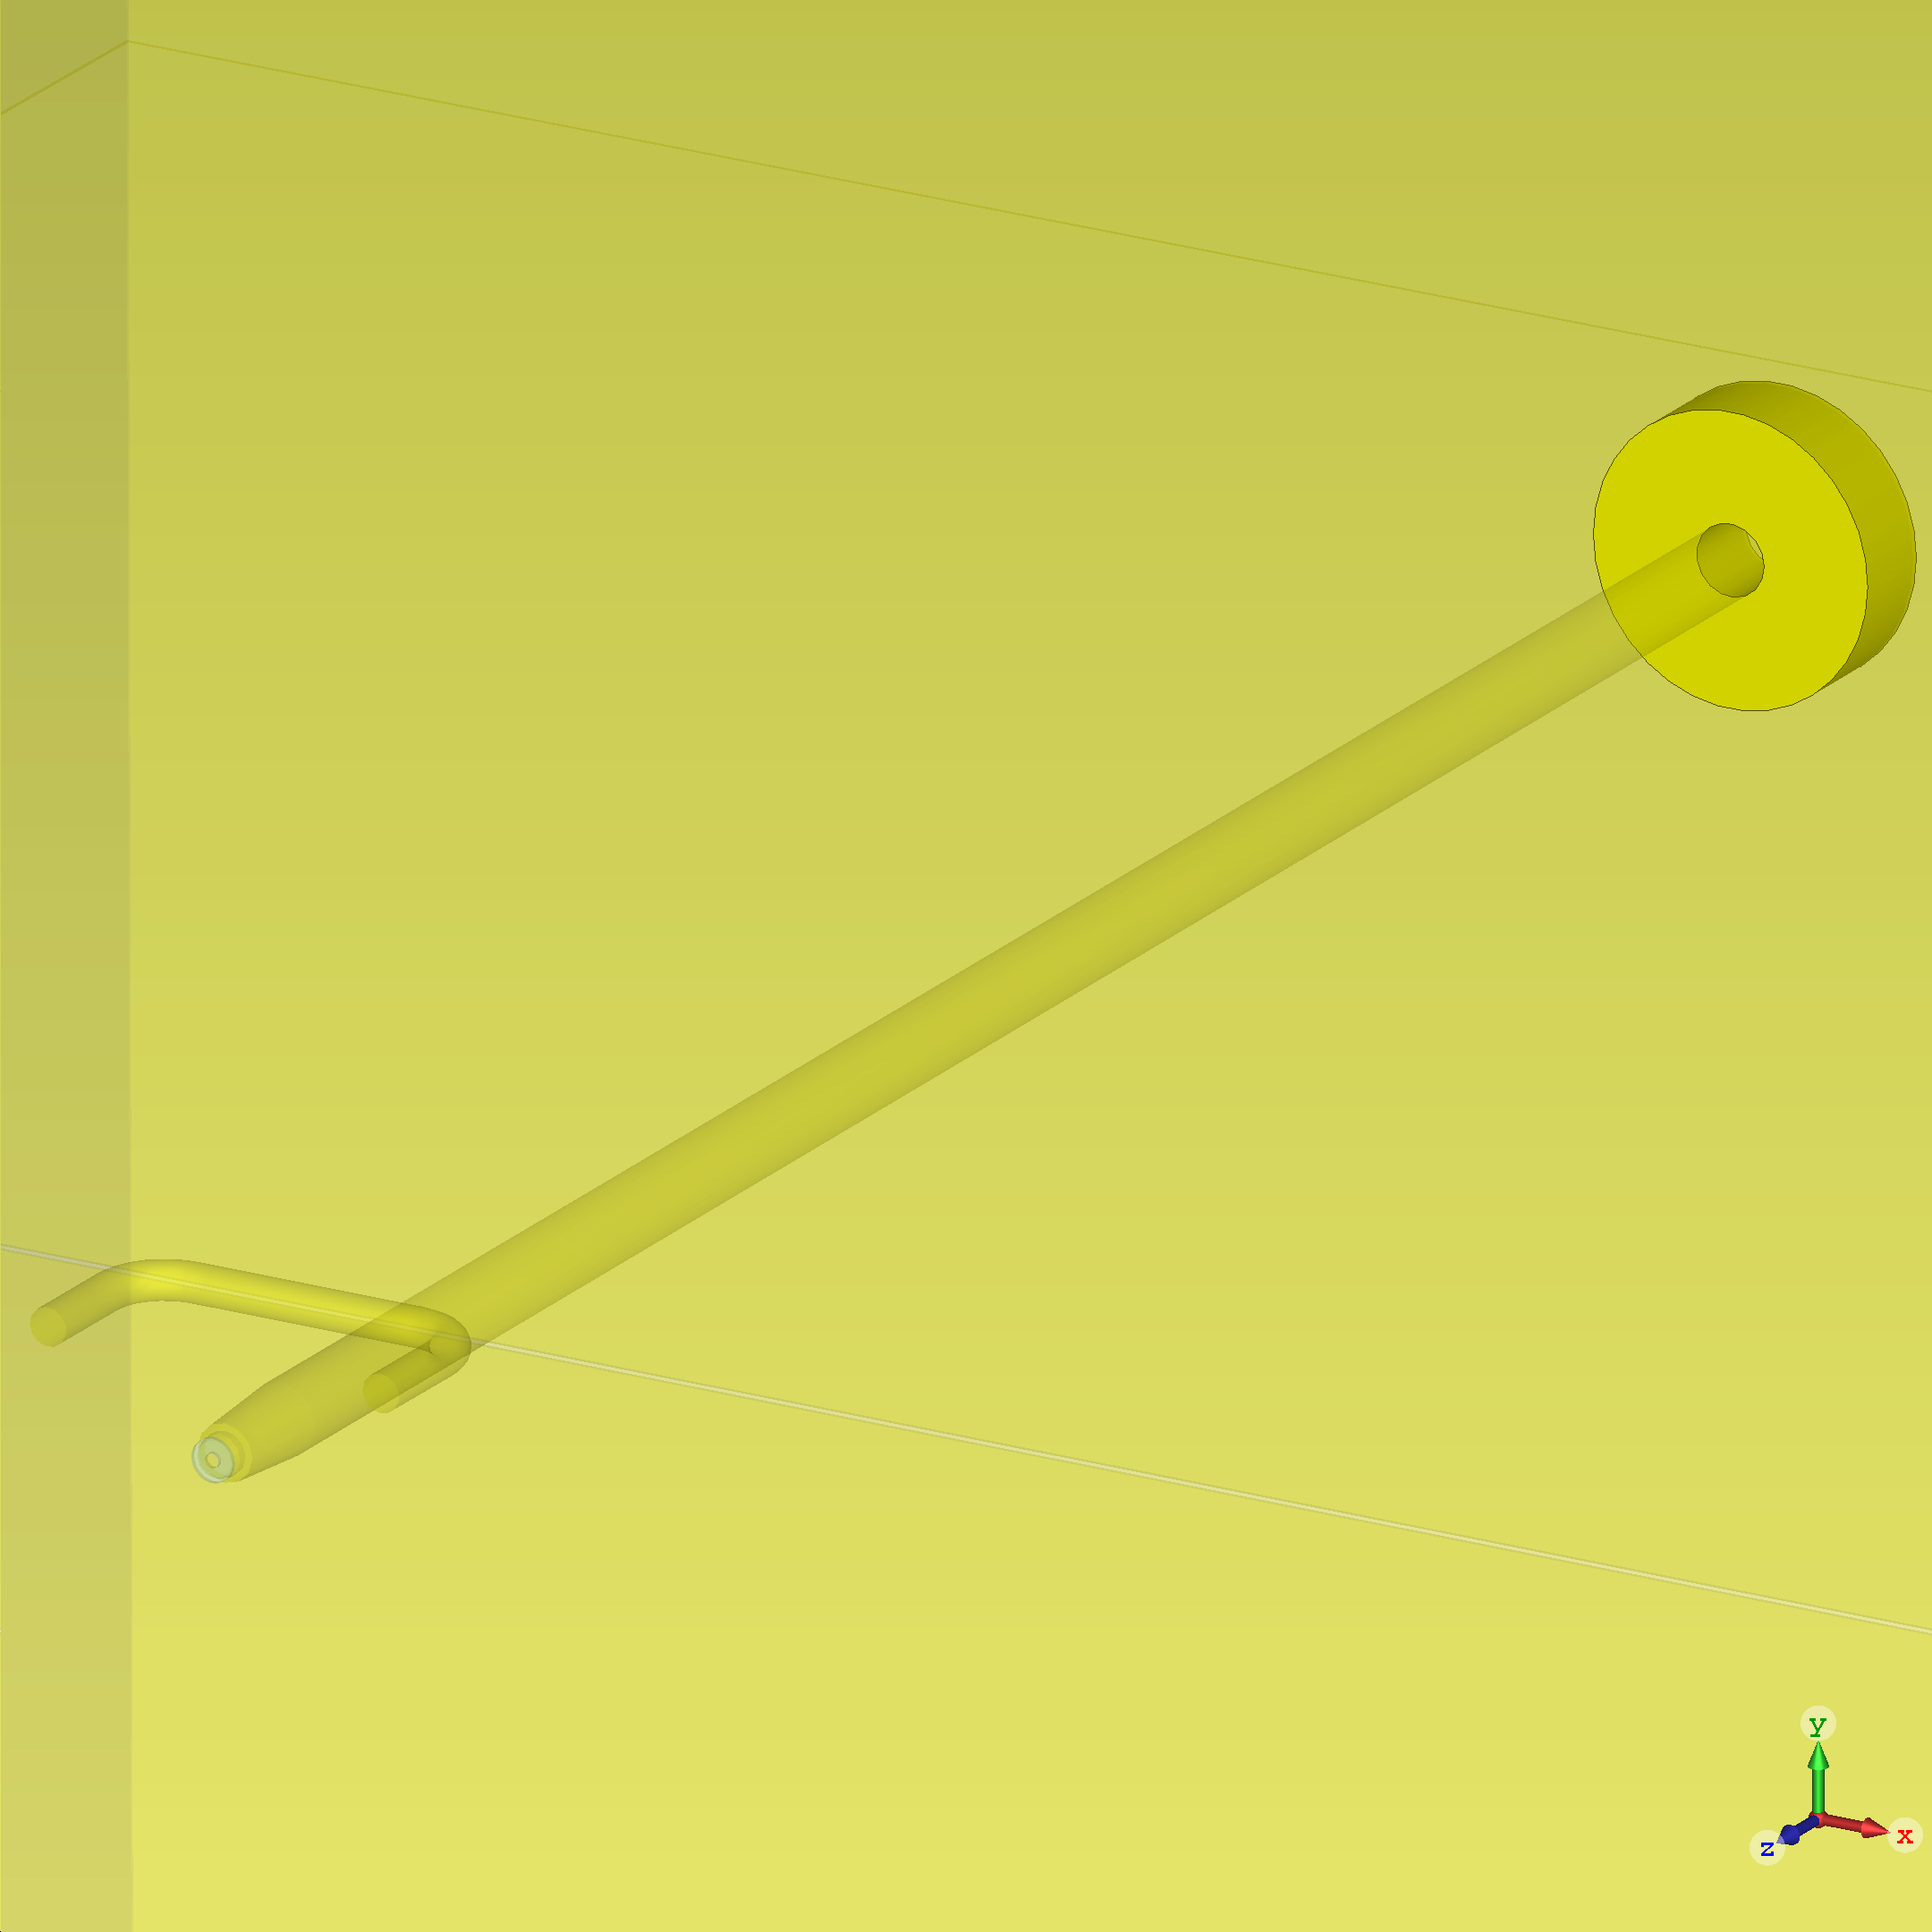
\includegraphics[height=0.3\textwidth]{./Simulation/Block.png}}
                \hspace{0.01\textwidth}
                \subfloat[Holzkonstruktion]{
                    \label{subfig:HolzKonst}
                    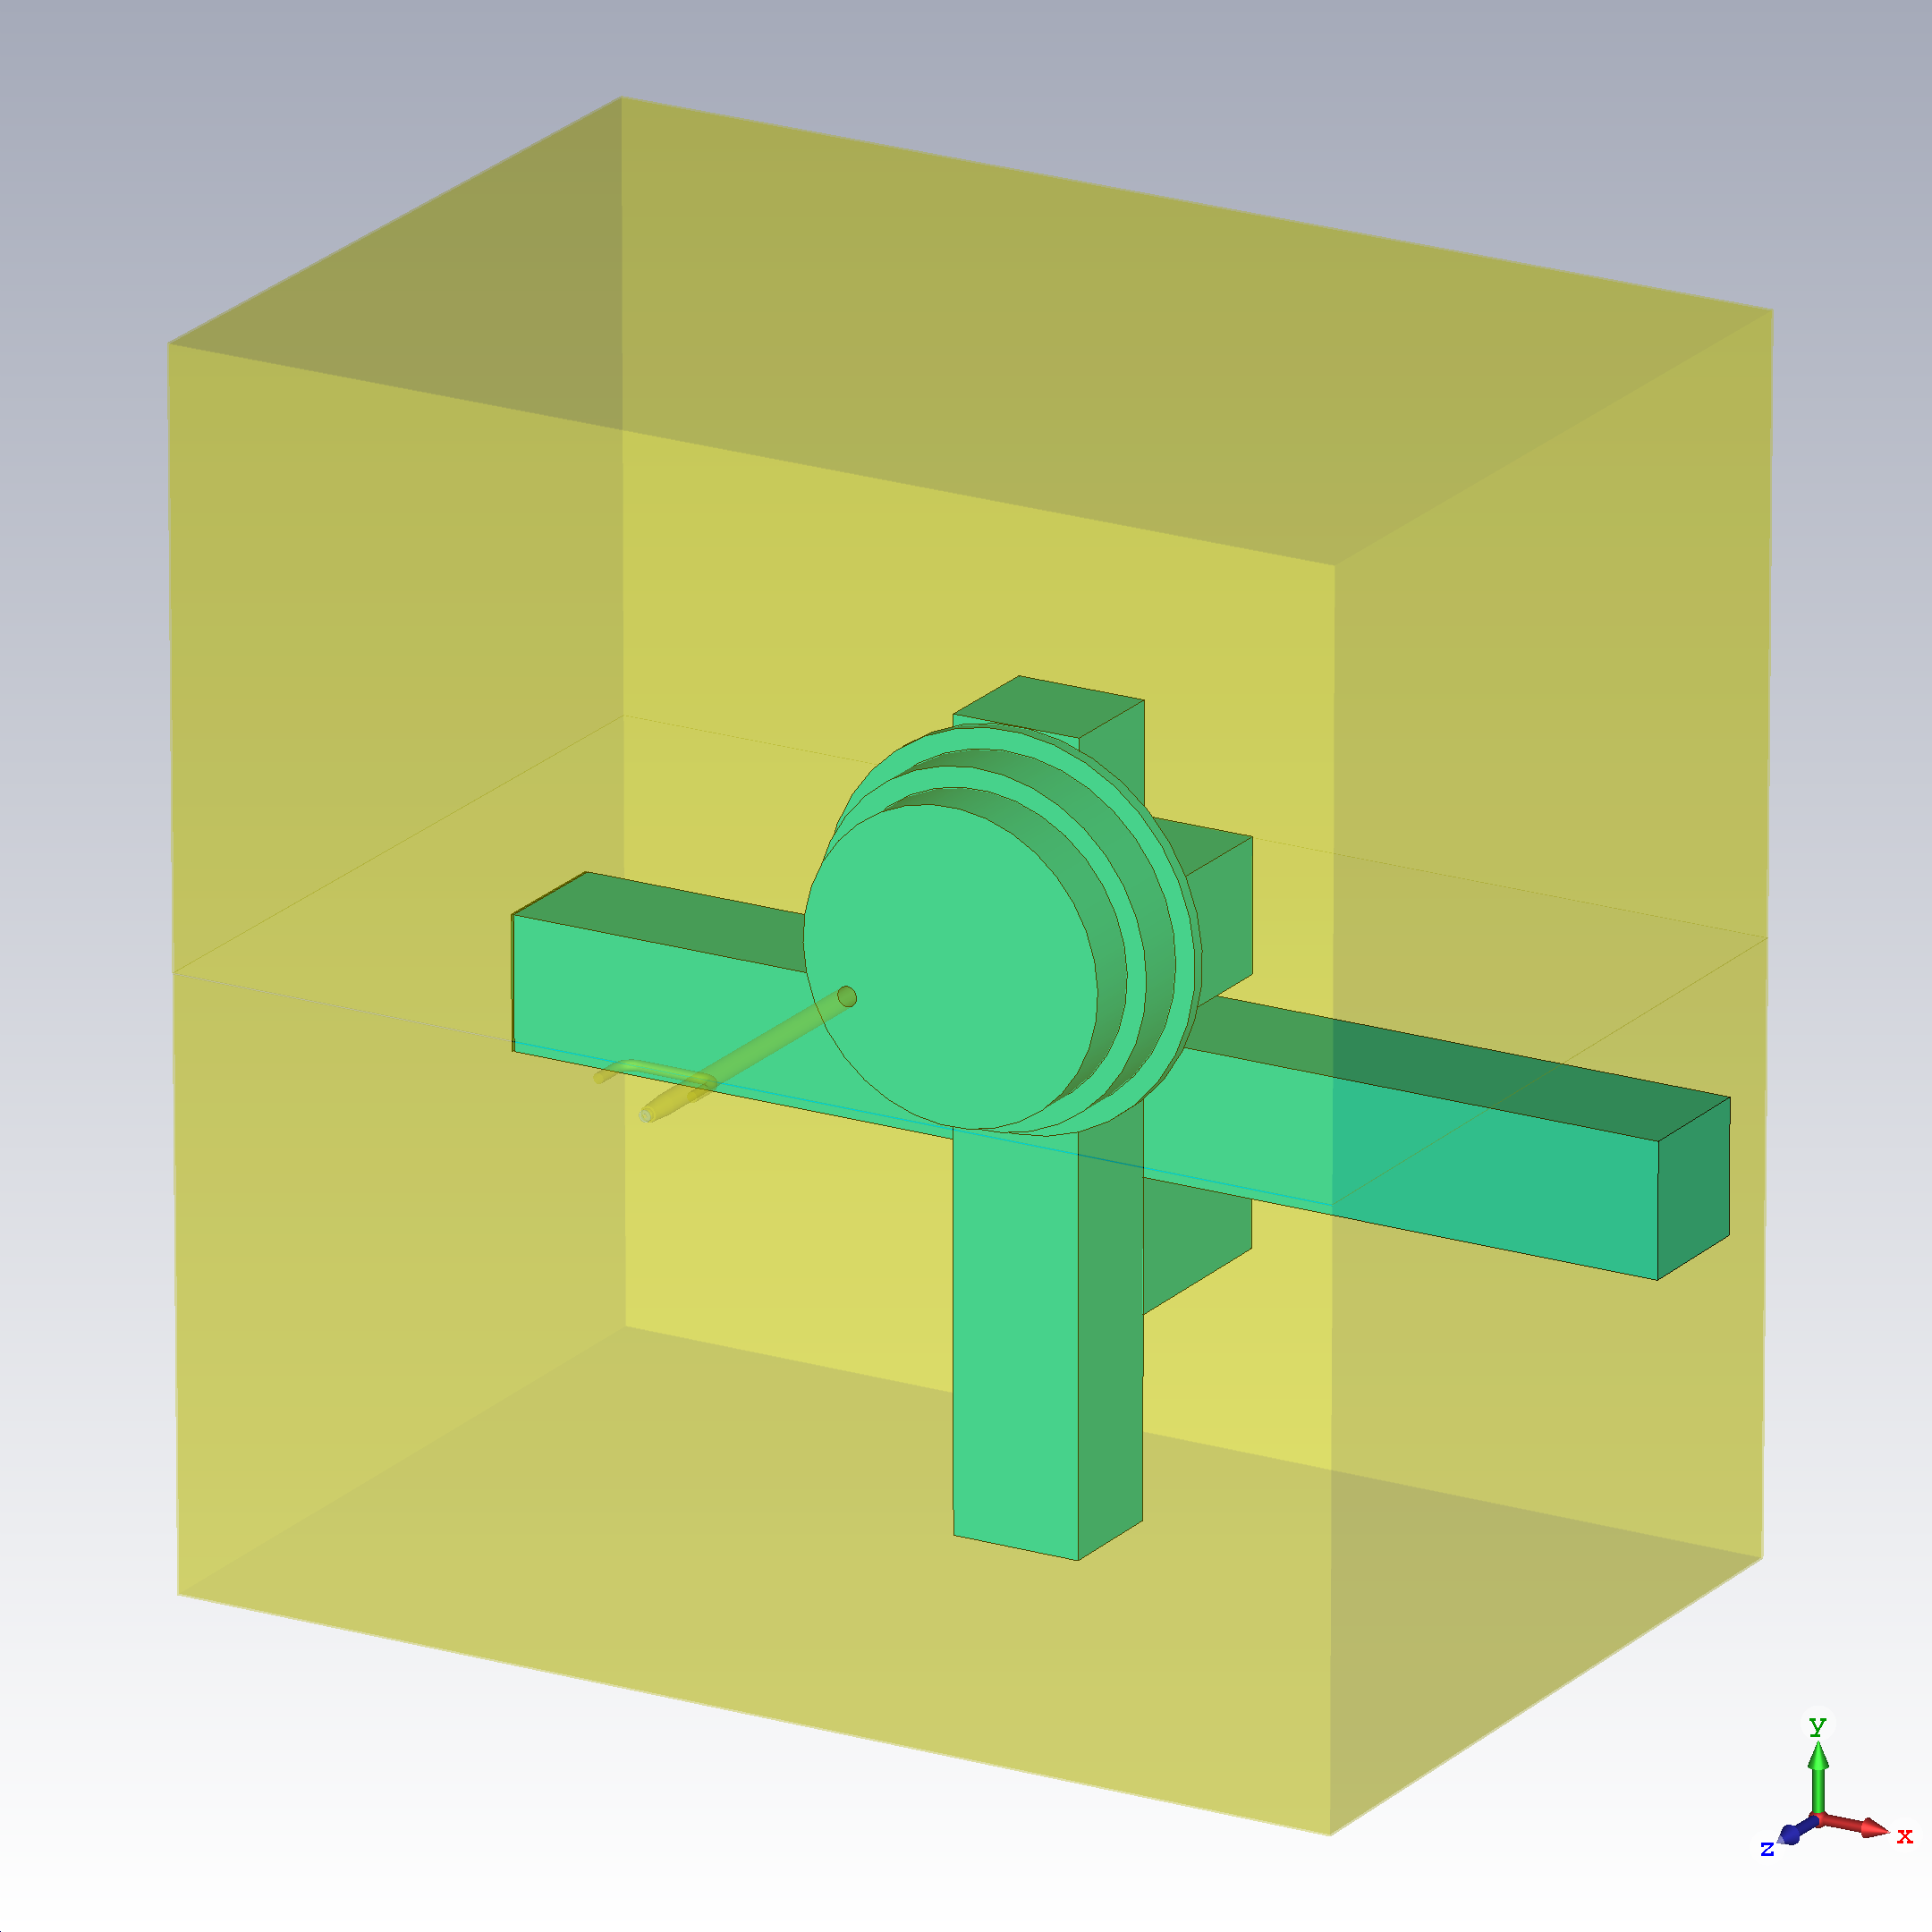
\includegraphics[height=0.3\textwidth]{./Simulation/HolzKonstrukt.png}}
                \caption{Anpassung des Simulationsmodells an den realen Aufbau \protect\subref{subfig:Buegel} Bügel über Einkopplung, \protect\subref{subfig:Block} Kupferzylinder an der Rückwand und \protect\subref{subfig:HolzKonst} die hölzerne Halterung des Ringkerns.}
                \label{fig:AnpassungCST}
            \end{figure}
        
            \subsubsection{Ringkern}
            \label{sec:ringkern}
            Die echten Ringkerne, wie sie bei der GSI benutzt werden, bestehen nicht nur aus dem MA-Material, sondern besitzen einen Innenkreis aus Eisen, der zur Montage dient. Da das Eisen andere magnetische Eigenschaften als das MA-Material besitzt, wurde dies in das Modell übernommen. Die neue Modellierung des Ringkerns mit innerem Eisenring ist in Abbildung~\ref{fig:RKFeRingCST} dargestellt.
                
                \begin{figure}[htb]
                    \centering
                    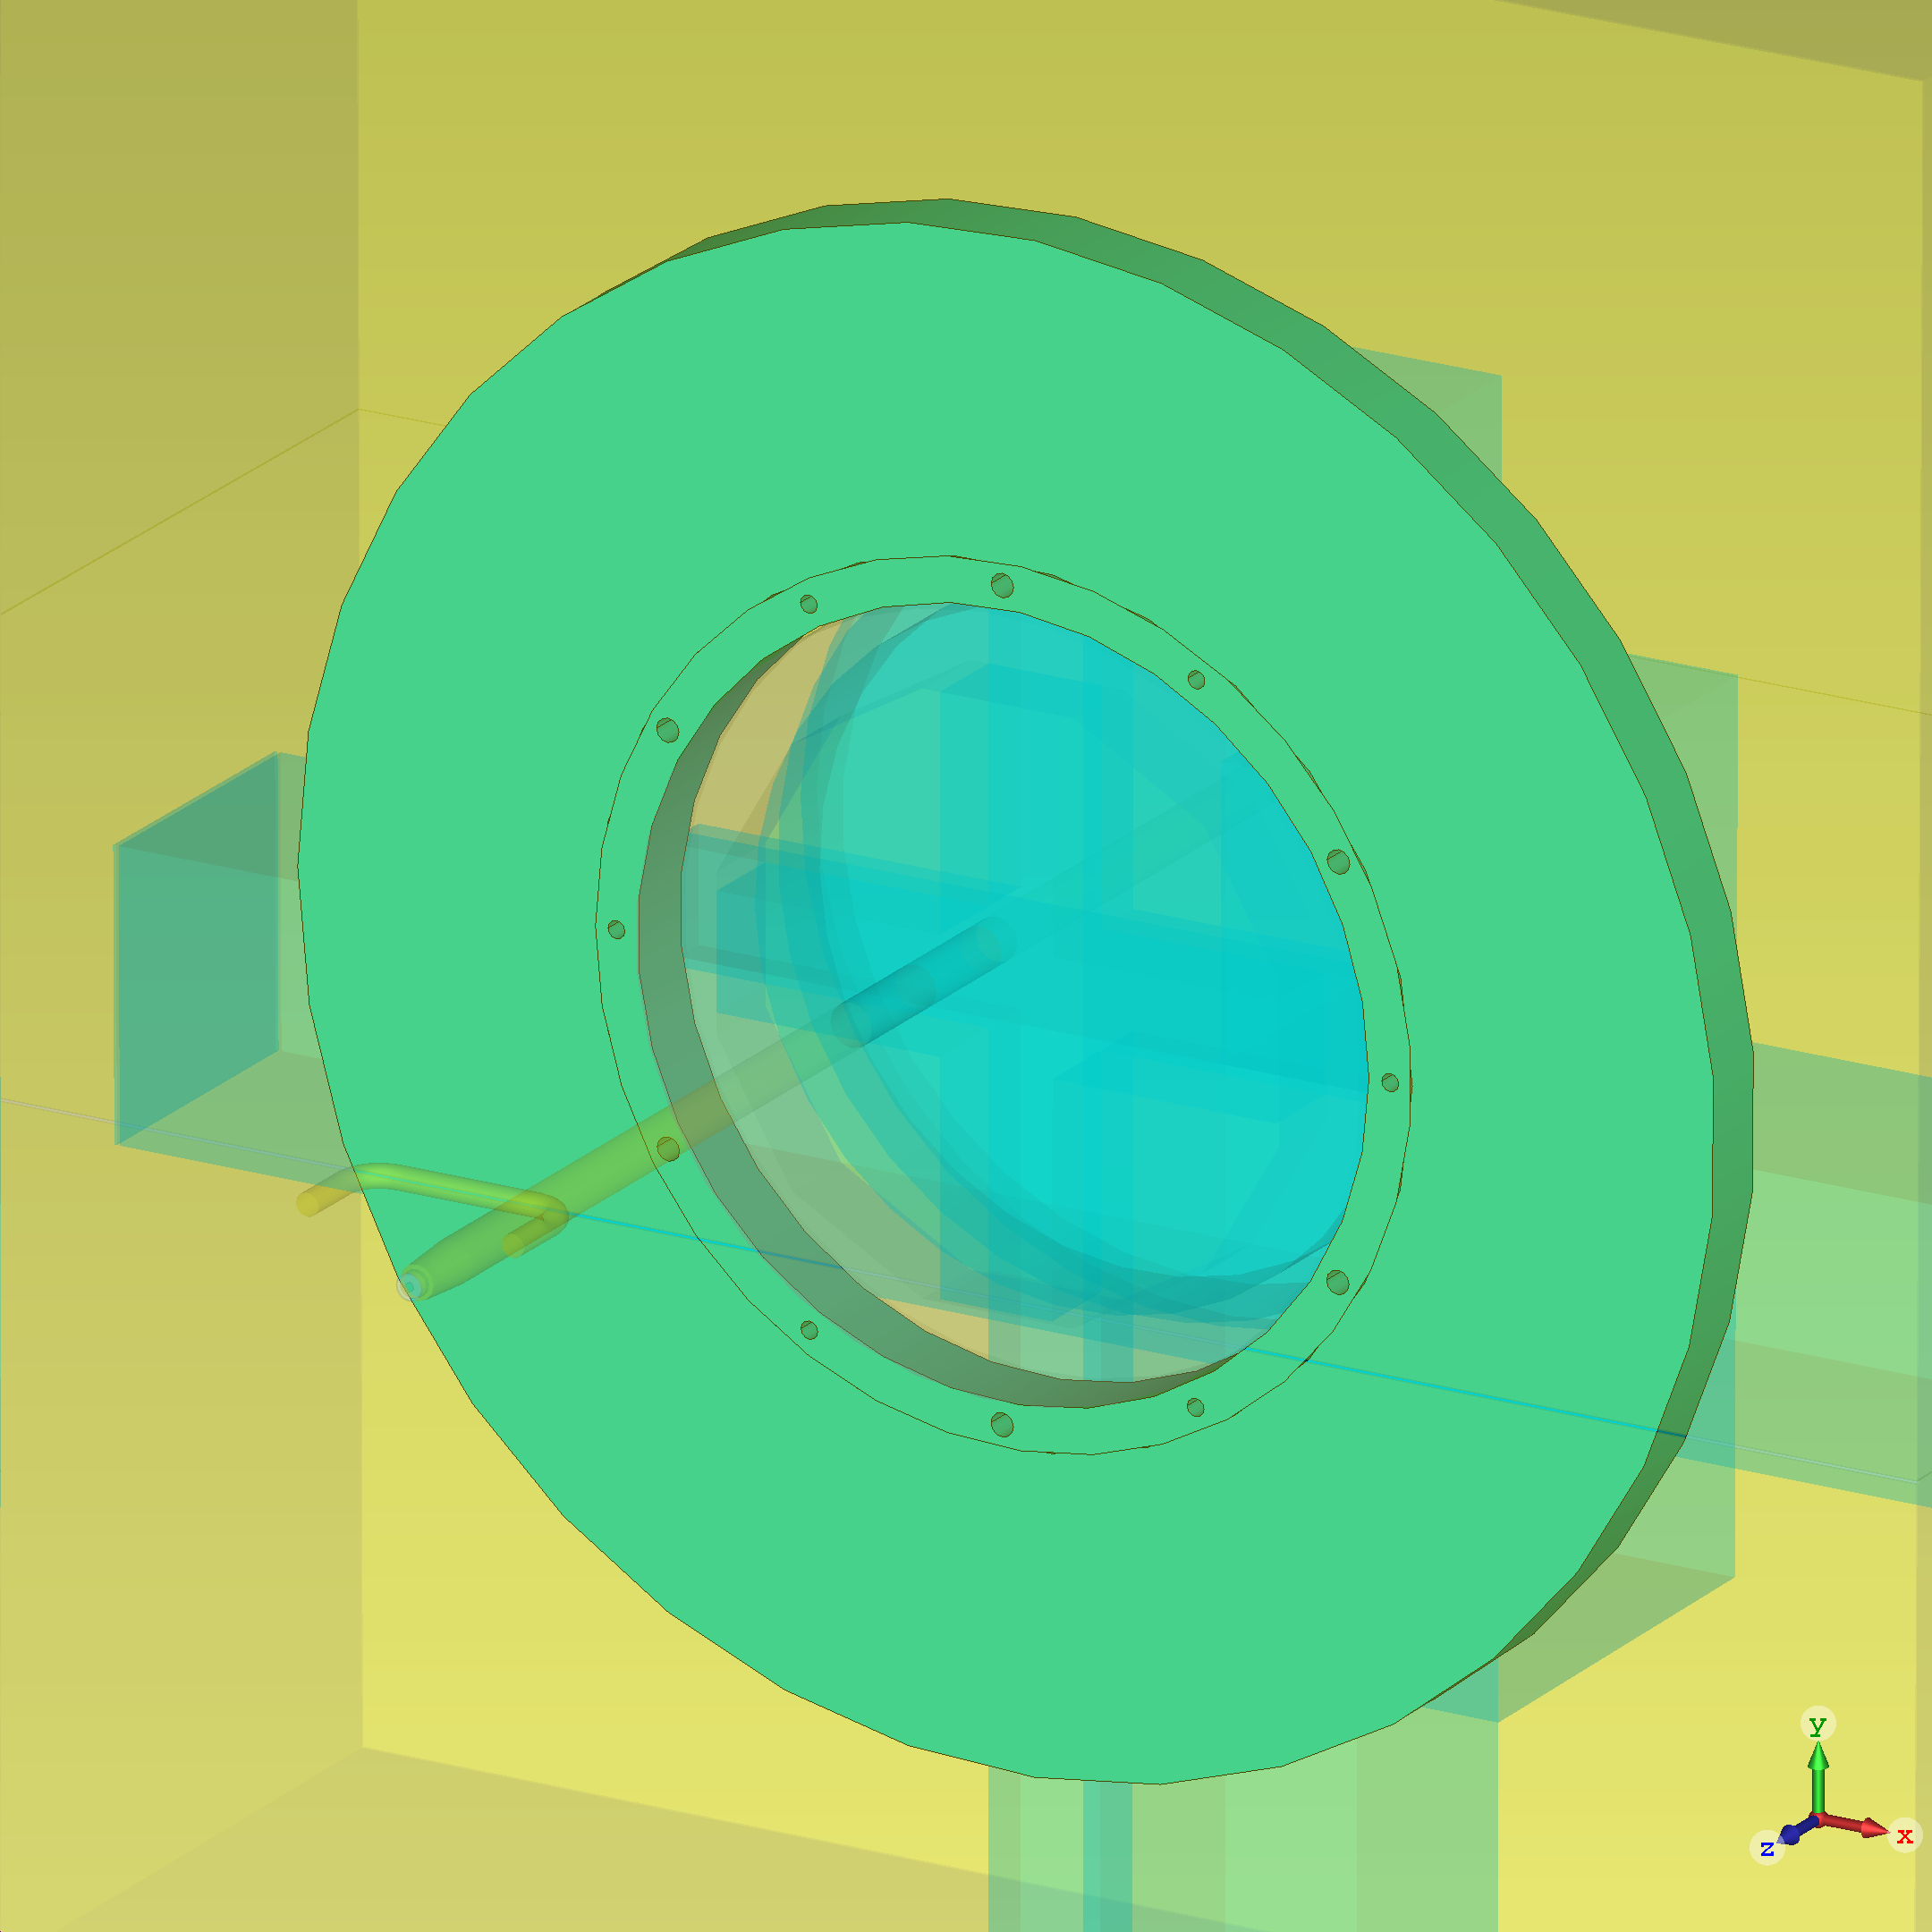
\includegraphics[height=0.4\textwidth]{./Simulation/RKFeRing.png}
                    \caption{Ringkernmodell mit innerem Eisenring}
                    \label{fig:RKFeRingCST}
                \end{figure}
            
            \par
            Des Weiteren wurde für eine bessere Übereinstimmung von Simulation und Messung die magnetische Permeabilität des Ringkernmaterials den Messungen entsprechend aktualisiert. Die Anpassung der Materialparameter basiert auf der Arbeit von Denys Bast~\citep{bast2017ba} und den theoretischen Grundlagen nach ~\citep{Klingbeil2008}.\\
            Die Testbox und der Ringkern können in ein Ersatzschaltbild überführt und damit der Impedanzverlauf analysiert werden. Das Ersatzschaltbild ist in Abbildung~\ref{fig:BoxRKCircuit} dargestellt, dabei wurde die Vorlage aus \citep{bast2017ba} um einen Widerstand ergänzt, der die Verluste der Anordnung nachbildet und für eine Dämpfung der Impedanzamplitude in Resonanz verantwortlich ist. Damit soll das hochfrequente Verhalten der Ersatzschaltung und der Messung besser in Übereinstimmung gebracht werden.\\
            Die Werte für die elektrischen Komponenten der Ersatzschaltung betragen:
                \begin{align}
                    R_{box} &= 16,46~k\Omega \nonumber\\
                    C_{box} &= 6,55~pF \nonumber\\
                    L_{box} &= 528,55~nH \nonumber
                \end{align}
            Die Impedanz dieser Anordnung bestimmt sich nach
                \begin{equation}\label{eq:Zges}
                    \underline{Z}_{ges} = \frac{R_{box}\cdot(\underline{Z}_{rk}+j\omega L_{box})}{R_{box}+(\underline{Z}_{rk}+j\omega L_{box})\cdot(1+j\omega R_{box}C_{box})}.
                \end{equation}
            Daraus lässt sich nun die Impedanz des Ringkerns $Z_{rk}$ bestimmen
                \begin{equation}\label{eq:Zrk}
                \underline{Z}_{rk} = \frac{\underline{Z}_{ges}\cdot(R_{box}+j\omega L_{box}-\omega^2\cdot R_{box}L_{box}C_{box}) - j\omega R_{box}L_{box}}{R_{box}-\underline{Z}_{ges}\cdot(1+j\omega R_{box}C_{box})}.
                \end{equation}
            Wird für $\underline{Z}_{ges}$ die Impedanz aus der Messung eingesetzt, kann die Ringkernimpedanz dieser Messung bestimmt werden.\\
            Nach~\citep{Klingbeil2008} kann diese als Reihenschaltung eines Widerstands $R_{rk}$ und einer Induktivität $L_{rk}$ als $\underline{Z}_{rk} = R_{rk}+j\omega L_{rk}$ betrachtet werden. Für das dissipative $\underline{\mu}_r = \mu' -j\mu''$  des Ringkerns wird in \citep{bast2017ba} angeführt, wie sich mittels der Ersatzschaltung $\mu'$ und $\mu''$ berechnen lassen:
                \begin{equation}
                    \mu' = \frac{L_{rk}\cdot 2\pi}{d\cdot ln\frac{r_a}{r_i}}
                \end{equation} 
                \begin{equation}
                \mu'' = \frac{R_{rk}\cdot\mu'}{\omega\cdot L_{rk}} .
                \end{equation}
            
                \begin{figure}[htb]
                    \centering
                    \begin{tikzpicture}
                    \node[above] at (-0.25,1.6) {$Z_{ges}$};
                    \draw (-0.5,1.4) -- (0.1,1.4);
                    \draw (-0.5,1.6) -- (0.1,1.6);
                    \path[fill=black, draw=black]
                        (0.1,1.3)  -- (0.1,1.7)  -- (0.5,1.5) --  (0.1,1.3);
                    \begin{circuitikz}
                    \draw
                    (2,0) to [resistor =$R_{box}$] (2,3)
                    (5,0) to [C, l=$C_{box}$] (5,3)
                    (5,3) to [L, l=$L_{box}$] (9,3)
                    (9,3) to [short, *-] (10,3)
                    (9,0) to [short, *-] (10,0)
                    (10,3) to [resistor =$Z_{rk}$] (10,0)
                    (0,3) to [short, *-] (5,3)
                    (0,0) to [short, *-] (5,0)
                    (8,3) to [short, -*] (9,3)
                    (5,0) to [short, -*] (9,0);
                    % 		(0,0) to [short, *- , i_=$I_5$] (1.5,-2);
                    \end{circuitikz}
                    \end{tikzpicture}
                    \caption{RLC-Ersatzschaltbild f\"ur die Testbox Modellierung mit Eingebrachtem Ringkern als Last.}
                    \label{fig:BoxRKCircuit}
                \end{figure}
                
            Ausgehend vom angepassten, dissipativen $\underline{\mu}_r$ kann nun die Simulation aktualisiert werden. Dazu werden die bestimmten Werte für $\mu'$ und $\mu''$ als Materialparameter in CST hinterlegt.
           
        \subsection{Erweiterung des Modells}
        Wie bereits in Kapitel~\ref{chap:messaufbau} erläutert, wurde die Testbox für die einfachere Montage der Kurzschlüsse und die erhöhte Reproduzierbarkeit der Messungen modifiziert und um ein kreuzförmiges Gestell aus Holz, sowie einen nichtleitenden Ring mit einem Polygonzug als Innenkreis erweitert (Geometrie und Beschreibung siehe Kapitel~\ref{chap:messaufbau}). Diese Modifikationen sind mit CST geometrisch genau nachgebildet (siehe Abb.~\ref{fig:KreuzPolygonCST}). Für das Holzkreuz wurden die selben Materialparameter verwendet, die für die Holzkreise hinterlegt sind, da es sich auch hierbei das Pressspanholz handelt.
        
            \begin{figure}[htb]
                \centering
                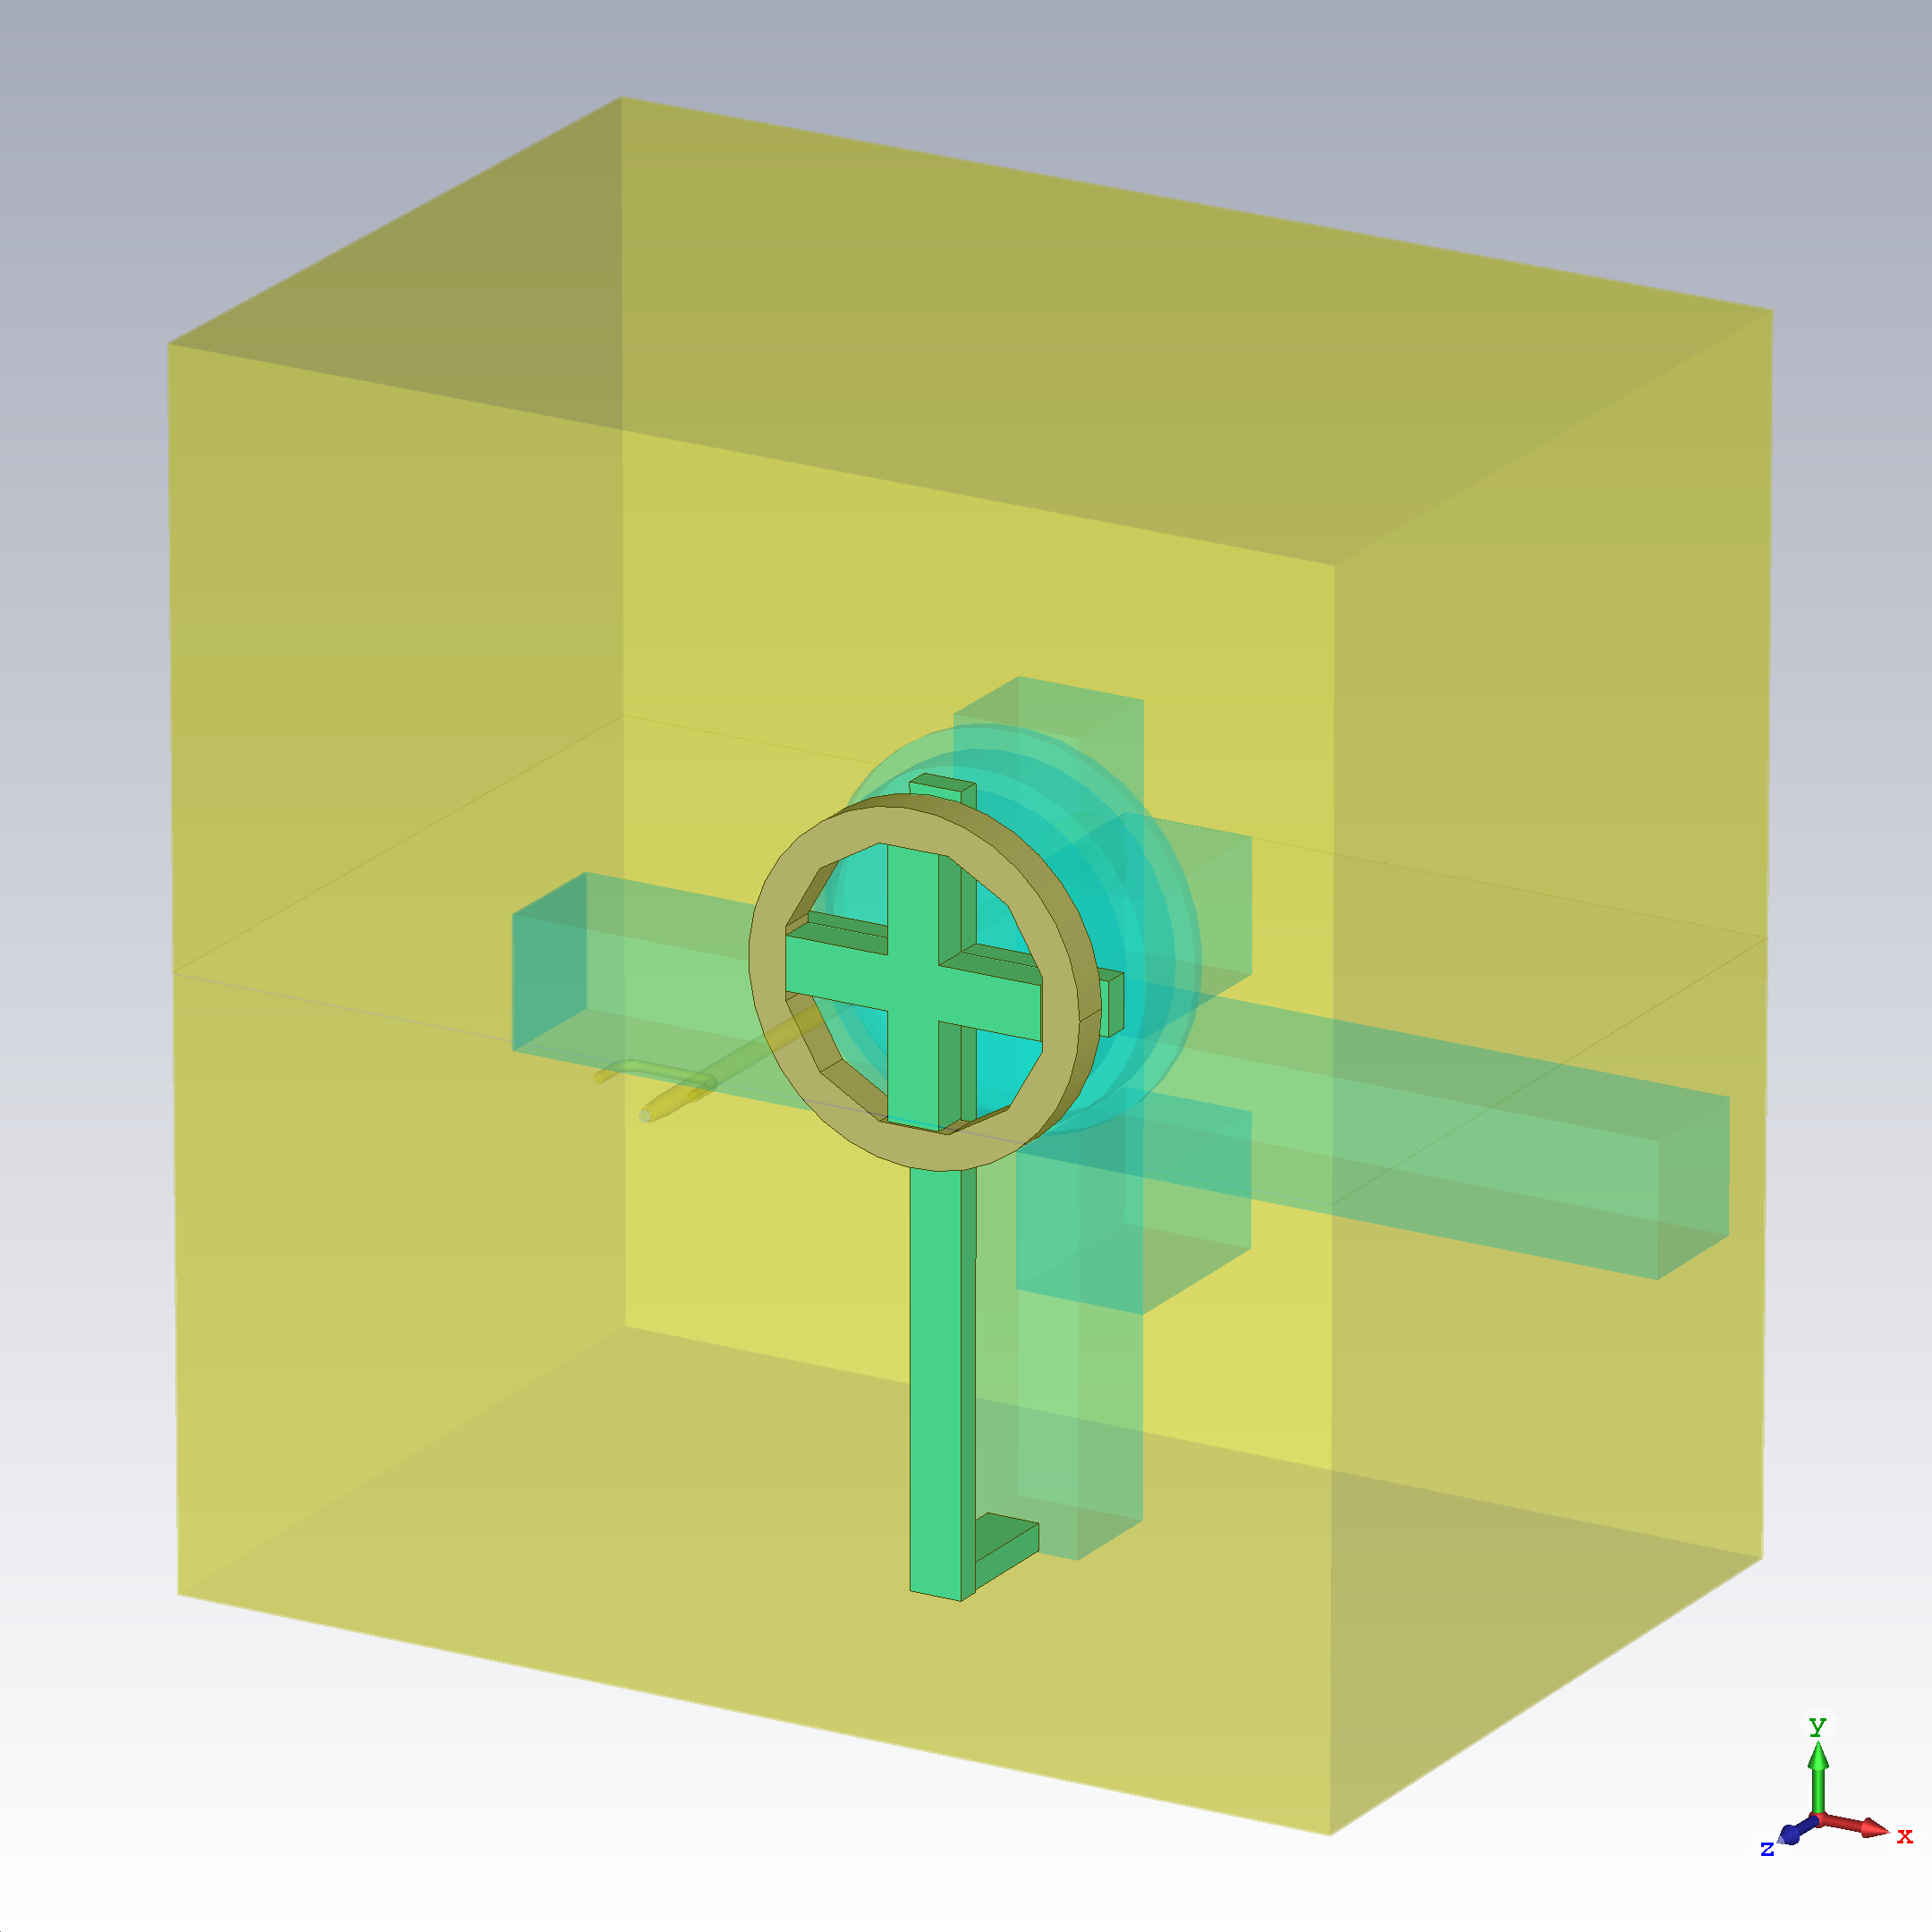
\includegraphics[height=0.4\textwidth]{./Simulation/KreuzPolygon.png}
                \caption{Erweiterung der Testbox um die Holzkreuzhalterung und den Polygonzug zur Befestigung der Kurzschlüsse}
                \label{fig:KreuzPolygonCST}
            \end{figure}
        
    \section{Durchführung}
    
    \todo[inline,color=red!30]{Hier weiter ausarbeiten!}
    
    \sout{Dieser Text soll nicht sein.}\textcolor{red}{Dieser Schon.}



\chapter{Plots}
	\section{Einfluss der Anzahl der Kurzschl\"usse}
F\"ur diese Analyse wurden Kurzschl\"usse mittels Torusringen um den Ringkern erzeugt. Dabei wurde sowohl die Anzahl, als auch die Position variiert. Abbildung~\ref{fig:AnzahlKs} zeigt die Einfl\"usse.
\begin{figure}[h]
	\centering
	\begin{tikzpicture}
		\begin{axis}[ymode = log, width=0.85\textwidth, height = 0.5\textwidth, xmin = 0.1, xmax = 100, xlabel=Frequenz in MHz, ylabel=Realteil der Impedanz der Kavit\"at in Ohm, xticklabel style={/pgf/number format/fixed,/pgf/number format/precision=5}, every axis plot/.append style={thick},every axis legend/.append style={at={(0.02,0.97)},anchor=north west}, grid=both, cycle list name=color list]
			\addplot table[x index=0,y index=1,mark=none] {../Inputfiles/plotData/Box.txt};
			\addplot table[x index=0,y index=1,mark=none] {../Inputfiles/plotData/Rk.txt};
			\addplot table[x index=0,y index=1,mark=none] {../Inputfiles/plotData/Rk1Ks0.txt};
			\addplot table[x index=0,y index=1,mark=none] {../Inputfiles/plotData/Rk4Ks90.txt};
			\addplot table[x index=0,y index=1,mark=none] {../Inputfiles/plotData/Rk24Ks15.txt};
			\legend{leere Box, Box mit Ringkern, 1 Kurzschluss, 4 Kurzschl\"usse (90 Grad versetzt),  24 Kurzschl\"usse}
		\end{axis}
	\end{tikzpicture}
	\caption{Verhaltend der Box ohne Ringkern im Vergleich zur Box mit Ringkern, sowie mit mehreren Kurzschl\"ussen}
	\label{fig:AnzahlKs}
\end{figure}

\newpage

\section{Einfluss der Positionierung der Kurzschl\"usse}
F\"ur diese Analyse werden 4 K\"urzschl\"usse einmal um 30 Grad versetzt um den Ringkern platziert, und einmal um 90 Grad versetzt.
\begin{figure}[h]
	\centering
	\begin{tikzpicture}
		\begin{axis}[ymode=log, width=0.85\textwidth, height = 0.5\textwidth, xmin = 0.1, xmax = 100, xlabel=Frequenz in MHz, ylabel=Realteil der Impedanz der Kavit\"at in Ohm, xticklabel style={/pgf/number format/fixed,/pgf/number format/precision=5}, every axis plot/.append style={thick},every axis legend/.append style={at={(0.02,0.97)},anchor=north west}, grid=both, cycle list name=color list]
			\addplot table[x index=0,y index=1,mark=none] {../Inputfiles/plotData/Box.txt};
			\addplot table[x index=0,y index=1,mark=none] {../Inputfiles/plotData/Rk.txt};
			\addplot table[x index=0,y index=1,mark=none] {../Inputfiles/plotData/Rk4Ks30.txt};
			\addplot table[x index=0,y index=1,mark=none] {../Inputfiles/plotData/Rk4Ks90.txt};
			\legend{leere Box, Box mit Ringkern, 4 Kurzschl\"usse (30 Grad versetzt), 4 Kurzschl\"usse (90 Grad versetzt)}
		\end{axis}
	\end{tikzpicture}
	\caption{Verhaltend der Box ohne Ringkern im Vergleich zur Box mit Ringkern, sowie mit mehreren Kurzschl\"ussen}
	\label{fig:PosKs}
\end{figure}

\newpage

\section{Einfluss der Form der Kurzschl\"usse}
F\"ur diese Analyse wird die Form der Kurzschl\"usse analysiert. Dazu wird wieder der einzelne Torus herangezogen und verglichen mit Verschieden breiten und weiten Kupferschienen. \\
\begin{figure}[h]
	\centering
	\begin{tikzpicture}
		\begin{axis}[ymode=log, width=0.85\textwidth, height = 0.5\textwidth, xmin = 0.1, xmax = 100, xlabel=Frequenz in MHz, ylabel=Realteil der Impedanz der Kavit\"at in Ohm, xticklabel style={/pgf/number format/fixed,/pgf/number format/precision=5}, every axis plot/.append style={thick},every axis legend/.append style={at={(0.02,0.97)},anchor=north west}, grid=both, cycle list name=color list]
			\addplot table[x index=0,y index=1,mark=none] {../Inputfiles/plotData/Box.txt};
			\addplot table[x index=0,y index=1,mark=none] {../Inputfiles/plotData/Rk.txt};
			\addplot table[x index=0,y index=1,mark=none] {../Inputfiles/plotData/Rk1Ks0.txt};
			\addplot table[x index=0,y index=1,mark=none] {../Inputfiles/plotData/Kupferschiene.txt};
			\addplot table[x index=0,y index=1,mark=none] {../Inputfiles/plotData/KupferschieneSchmal.txt};
			\legend{leere Box, Box mit Ringkern, 1 Kurzschluss(Torus), 1 Kupferschiene, 1 Kupferschiene (schmal)}
		\end{axis}
	\end{tikzpicture}
	\caption{Verhaltend der Box ohne Ringkern im Vergleich zur Box mit Ringkern, sowie mit mehreren Kurzschl\"ussen}
	\label{fig:FormKs}
\end{figure}

\newpage

Des Weiteren wird der Vergleich mit mehreren Kurzschl\"ussen gezogen. Hierbei werden 4 Toruskurzschl\"usse 4 Kupferschienenkurzschl\"ussen gegen\"uber gestellt.
\begin{figure}[h]
	\centering
	\begin{tikzpicture}
		\begin{axis}[ymode=log, width=0.85\textwidth, height = 0.5\textwidth, xmin = 0.1, xmax = 100, xlabel=Frequenz in MHz, ylabel=Realteil der Impedanz der Kavit\"at in Ohm, xticklabel style={/pgf/number format/fixed,/pgf/number format/precision=5}, every axis plot/.append style={thick},every axis legend/.append style={at={(0.02,0.97)},anchor=north west}, grid=both, cycle list name=color list]
			\addplot table[x index=0,y index=1,mark=none] {../Inputfiles/plotData/Box.txt};
			\addplot table[x index=0,y index=1,mark=none] {../Inputfiles/plotData/Rk.txt};
			\addplot table[x index=0,y index=1,mark=none] {../Inputfiles/plotData/Rk4Ks90.txt};
			\addplot table[x index=0,y index=1,mark=none] {../Inputfiles/plotData/Kupferschiene4x.txt};
			\legend{leere Box, Box mit Ringkern, 4 Kurzschl\"usse(Torus), 4 Kupferschienen}
		\end{axis}
	\end{tikzpicture}
	\caption{Verhaltend der Box ohne Ringkern im Vergleich zur Box mit Ringkern, sowie mit mehreren Kurzschl\"ussen}
	\label{fig:Form4Ks}
\end{figure}

\newpage

\section{Einfluss des Abstands der Kurzschl\"usse vom Ringkern}
\begin{figure}[h]
	\centering
	\begin{tikzpicture}
		\begin{axis}[ymode=log, width=0.85\textwidth, height = 0.5\textwidth, xmin = 0.1, xmax = 100, xlabel=Frequenz in MHz, ylabel=Realteil der Impedanz der Kavit\"at in Ohm, xticklabel style={/pgf/number format/fixed,/pgf/number format/precision=5}, every axis plot/.append style={thick},every axis legend/.append style={at={(0.32,0.4)},anchor=north west}, grid=both, cycle list name=color list]
			\addplot table[x index=0,y index=1,mark=none] {../Inputfiles/plotData/Box.txt};
			\addplot table[x index=0,y index=1,mark=none] {../Inputfiles/plotData/Rk.txt};
			\addplot table[x index=0,y index=1,mark=none] {../Inputfiles/plotData/Kupferschiene.txt};
			\addplot table[x index=0,y index=1,mark=none] {../Inputfiles/plotData/KupferschieneAbstandsvariation.txt};
			\addplot table[x index=0,y index=1,mark=none] {../Inputfiles/plotData/KupferschieneEngRK.txt};
			\legend{leere Box, Box mit Ringkern, 1 Kupferschiene, 1 Kupferschiene (weiter Abstand von Ringkern, 1 Kupferschiene (eng am Ringkern)}
		\end{axis}
	\end{tikzpicture}
	\caption{Verhaltend der Box ohne Ringkern im Vergleich zur Box mit Ringkern, sowie mit mehreren Kurzschl\"ussen}
	\label{fig:FormKs}
\end{figure}

\newpage

\section{Einfluss im Falle einer passiven Schiene}
Bei einer Schiene:
\begin{figure}[h]
	\centering
	\begin{tikzpicture}
		\begin{axis}[ymode=log, width=0.85\textwidth, height = 0.5\textwidth, xmin = 0.1, xmax = 100, xlabel=Frequenz in MHz, ylabel=Realteil der Impedanz der Kavit\"at in Ohm, xticklabel style={/pgf/number format/fixed,/pgf/number format/precision=5}, every axis plot/.append style={thick},every axis legend/.append style={at={(0.02,0.97)},anchor=north west}, grid=both, cycle list name=color list]
			\addplot table[x index=0,y index=1,mark=none] {../Inputfiles/plotData/Rk.txt};
			\addplot table[x index=0,y index=1,mark=none] {../Inputfiles/plotData/KupferschieneOffen.txt};
			\legend{Box mit Ringkern, Box mit einer Offenen Kupferschiene}
		\end{axis}
	\end{tikzpicture}
	\caption{Verhaltend der Box mit Ringkern im Vergleich zur Box mit einer offenen Kupferschiene}
	\label{fig:passiv}
\end{figure}

\newpage

Bei mehreren Schienen:
\begin{figure}[h]
	\centering
	\begin{tikzpicture}
		\begin{axis}[ymode=log, width=0.85\textwidth, height = 0.5\textwidth, xmin = 0.1, xmax = 100, xlabel=Frequenz in MHz, ylabel=Realteil der Impedanz der Kavit\"at in Ohm, xticklabel style={/pgf/number format/fixed,/pgf/number format/precision=5}, every axis plot/.append style={thick},every axis legend/.append style={at={(0.02,0.97)},anchor=north west}, grid=both, cycle list name=color list]
			\addplot table[x index=0,y index=1,mark=none] {../Inputfiles/plotData/Rk.txt};
			\addplot table[x index=0,y index=1,mark=none] {../Inputfiles/plotData/KupferschieneOffen4x.txt};
			\legend{Box mit Ringkern, Box mit vier offenen Kupferschienen}
		\end{axis}
	\end{tikzpicture}
	\caption{Verhaltend der Box mit Ringkern im Vergleich zur Box mit einer offenen Kupferschiene}
	\label{fig:passiv}
\end{figure}
	
%% Appendix %%%%%%%%%%%%%%%%%%%%%%%%%%%%%%%%%%%%%%%%%%%%%%%%%%%%%%%%%%%%%%%%
\pagestyle{plain}
\appendix
\newcommand{\hiddensection}[1]{
    \stepcounter{section}
    \section*{\Alph{chapter}.\arabic{section}\hspace{0.8em}{#1}}
}
\chapter{Appendix: --}
%    \input{../Inputfiles/Chapters/_.tex}
\cleardoublepage

%% Literatur %%%%%%%%%%%%%%%%%%%%%%%%%%%%%%%%%%%%%%%%%%%%%%%%%%%%%%%%%%%%%%%
\bibliographystyle{plain}
%\bibliography{../Inputfiles/Literature/_.bib}
\cleardoublepage

%% Tabellen und Abbildungen %%%%%%%%%%%%%%%%%%%%%%%%%%%%%%%%%%%%%%%%%%%%%%%%
% List of figures:
\listoffigures
\cleardoublepage

% List of tables:
\listoftables
\cleardoublepage

\end{document}